\documentclass[11pt]{article}
%\usepackage{lipsum,mathptmx,etoolbox} % Or swap mathptmx with newtxtext,newtxmath
\usepackage[utf8]{inputenc}
\usepackage[french,english]{babel}
\usepackage[autostyle,french=guillemets*]{csquotes} % needed for babel
\usepackage{fancyhdr, graphicx} % headeres, footeres, etc.. (see \fancypagestyle control sequence)
\usepackage{listings} % source code listings
\usepackage{hyperref} % Link citations with references at the end
\usepackage{url} % make links clickable
% \usepackage{cite} % nicht kompatibel mit biblatex

% Text
%\usepackage{color} % superseeded by xcolor
\usepackage{xcolor} % superseeds color
\usepackage[font=it]{caption} % Captions
\usepackage{subcaption} % captions for figures and the like
%\usepackage[scaled=0.92]{helvet}
\def\code#1{\texttt{#1}} % shortcut for monospaced inline code
\usepackage{makecell} % tables
\renewcommand{\familydefault}{\rmdefault}
%An initial of the very first character of the content
%\usepackage{lettrine}
%\newcommand{\initial}[1]{%
%	\lettrine[lines=2,lhang=0.33,nindent=0em]{
%		\color{gray}
%		{\textsc{#1}}}{}}

% Page layout
\usepackage[a4paper,top=2cm]{geometry}
\usepackage{enumitem} % control layout of itemize, enumerate, description
\usepackage{parskip}
\setlength{\textwidth}{17cm}
\setlength{\headheight}{27pt}
\setlength{\oddsidemargin}{-0.5cm}
\usepackage{lastpage} % for getting last page number
%\renewcommand{\familydefault}{\sfdefault}
\usepackage{setspace} % line space
\usepackage{acronym} % acronym index
%\numberwithin{equation}{section} %Metadata
\usepackage[export]{adjustbox}

% Tables
\usepackage{array}
\usepackage{booktabs}
\newcommand{\ra}[1]{\renewcommand{\arraystretch}{#1}}
\usepackage{colortbl}

% Bibliography
\usepackage[backend=biber,style=authoryear,citestyle=authoryear]{biblatex}
\addbibresource{./mybib.bib} %biblatex

% Math
\usepackage{amsmath}
\usepackage{amsfonts}
\usepackage{amssymb}
\usepackage{amsthm}

% Source code listings (coconfiguration of \usepackage{listings})

\DeclareCaptionFont{white}{\color{white}}
\DeclareCaptionFormat{listing}{\colorbox{gray}{\parbox{\textwidth}{#1#2#3}}}
%\captionsetup[lstlisting]{format=listing,labelfont=white,textfont=white}
\lstset{
% language=Python,
 basicstyle=\footnotesize\ttfamily, % Standardschrift
 captionpos=b,
% numbers=left,               % Ort der Zeilennummern
 numberstyle=\tiny,          % Stil der Zeilennummern
% stepnumber=5,              % Abstand zwischen den Zeilennummern
% numbersep=5pt,              % Abstand der Nummern zum Text
% tabsize=2,                  % Groesse von Tabs
% extendedchars=true,         %
 breaklines=true,            % Zeilen werden Umgebrochen
% frame=b,
 %commentstyle=\itshape\color{LightLime}, Was isch das? O_o
 %keywordstyle=\bfseries\color{DarkPurple}, und das O_o
% basicstyle=\small,
% stringstyle=\color[RGB]{42,0,255}\ttfamily, % Farbe der String
% keywordstyle=\color[RGB]{127,0,85}\ttfamily, % Farbe der Keywords
% commentstyle=\color[RGB]{63,127,95}\ttfamily, % Farbe des Kommentars
% showspaces=false,           % Leerzeichen anzeigen ?
% showtabs=false,             % Tabs anzeigen ?
% xleftmargin=17pt,
% framexleftmargin=17pt,
% framexrightmargin=5pt,
% framexbottommargin=4pt,
% showstringspaces=false,      % Leerzeichen in Strings anzeigen ?
 literate=
 {á}{{\'a}}1 {é}{{\'e}}1 {í}{{\'i}}1 {ó}{{\'o}}1 {ú}{{\'u}}1
 {Á}{{\'A}}1 {É}{{\'E}}1 {Í}{{\'I}}1 {Ó}{{\'O}}1 {Ú}{{\'U}}1
 {à}{{\`a}}1 {è}{{\`e}}1 {ì}{{\`i}}1 {ò}{{\`o}}1 {ù}{{\`u}}1
 {À}{{\`A}}1 {È}{{\'E}}1 {Ì}{{\`I}}1 {Ò}{{\`O}}1 {Ù}{{\`U}}1
 {ä}{{\"a}}1 {ë}{{\"e}}1 {ï}{{\"i}}1 {ö}{{\"o}}1 {ü}{{\"u}}1
 {Ä}{{\"A}}1 {Ë}{{\"E}}1 {Ï}{{\"I}}1 {Ö}{{\"O}}1 {Ü}{{\"U}}1
 {â}{{\^a}}1 {ê}{{\^e}}1 {î}{{\^i}}1 {ô}{{\^o}}1 {û}{{\^u}}1
 {Â}{{\^A}}1 {Ê}{{\^E}}1 {Î}{{\^I}}1 {Ô}{{\^O}}1 {Û}{{\^U}}1
 {œ}{{\oe}}1 {Œ}{{\OE}}1 {æ}{{\ae}}1 {Æ}{{\AE}}1 {ß}{{\ss}}1
 {ű}{{\H{u}}}1 {Ű}{{\H{U}}}1 {ő}{{\H{o}}}1 {Ő}{{\H{O}}}1
 {ç}{{\c c}}1 {Ç}{{\c C}}1 {ø}{{\o}}1 {å}{{\r a}}1 {Å}{{\r A}}1
 {€}{{\euro}}1 {£}{{\pounds}}1 {«}{{\guillemotleft}}1
 {»}{{\guillemotright}}1 {ñ}{{\~n}}1 {Ñ}{{\~N}}1 {¿}{{?`}}1
}

% Page Styles
\fancypagestyle{firststyle}{ %Style of the first page
 \fancyhf{}
 \fancyheadoffset[L]{0.6cm}
 \lhead{
\includegraphics[scale=0.8,valign=M]{./img/fhnw_logo.jpg}}
 \rhead{
\includegraphics[scale=0.3,valign=M]{./img/mse_logo.jpg}}
 \renewcommand{\headrulewidth}{0pt}
 \lfoot{Institute for Data Science,\linebreak www.fhnw.ch }
}

\fancypagestyle{documentstyle}{ %Style of the rest of the document
 \fancyhf{}
 \fancyheadoffset[L]{0.6cm}
 \lhead{
\includegraphics[scale=0.8,valign=M]{./img/fhnw_logo.jpg}}
 \rhead{
\includegraphics[scale=0.3,valign=M]{./img/mse_logo.jpg}}
 \renewcommand{\headrulewidth}{0pt}
 \lfoot{Speech-To-Text Engine for Forced Alignment}
 \rfoot{\thepage\ / \pageref{LastPage} }
}

\fancypagestyle{tableofcontent}{ %Style of the rest of the document
 \fancyhf{}
 \fancyheadoffset[L]{0.6cm}
 \lhead{
\includegraphics[scale=0.8,valign=M]{./img/fhnw_logo.jpg}}
 \rhead{
\includegraphics[scale=0.3,valign=M]{./img/mse_logo.jpg}}
 \renewcommand{\headrulewidth}{0pt}
 \cfoot{\thepage}
}

\fancypagestyle{abstract}{ %Style of the first page
 \fancyhf{}
 \fancyheadoffset[L]{0.6cm}
 \lhead{
\includegraphics[scale=0.8,valign=M]{./img/fhnw_logo.jpg}}
 \rhead{
\includegraphics[scale=0.3,valign=M]{./img/mse_logo.jpg}}
 \renewcommand{\headrulewidth}{0pt}
 \cfoot{}
}

\begin{document}
\begin{titlepage}
\vspace*{13mm}
\begin{center}
	\rule[0.5ex]{\linewidth}{2pt}\vspace*{-\baselineskip}\vspace*{3.2pt}
	\rule[0.5ex]{\linewidth}{1pt}\\[\baselineskip]
	
\includegraphics[scale=0.4]{./img/mse_logo.jpg}\\[4mm]
	{\huge Speech-To-Text Engine for Forced Alignment }\\[4mm]
	{\Large \textit{Master Thesis}}\\
	\rule[0.5ex]{\linewidth}{1pt}\vspace*{-\baselineskip}\vspace{3.2pt}
	\rule[0.5ex]{\linewidth}{2pt}\\
	\vspace{6.5mm}
	{\large By}\\
	\vspace{6.5mm}
	{\large\textsc{Daniel Tiefenauer}}\\
	daniel.tiefenauer@students.fhnw.ch\\
	\vspace{11mm}
	
\includegraphics{./img/fhnw_logo.jpg} \\
	\vspace{6mm}
	{\large Institute for Data Science (I4DS)}\\
	\vspace{11mm}
	\begin{minipage}{10cm}
		\begin{tabular}{ll}
			\textbf{Advisor} & Manfred Vogel (manfred.vogel@fhnw.ch) \\
			\textbf{Expert} & Mark Cieliebak (mark.cieliebak@zhaw.ch) \\
			\textbf{Industry Partner} & ReadyLingua \\
 			& Ulrike Glavitsch (ulrike.glavitsch@gmail.com)
		\end{tabular}
	\end{minipage}\\
	\vspace{9mm}
	{\large\textsc{December 3, 2018}}
	\vspace{12mm}
\end{center}
\end{titlepage}
%\title{IP9}
%\author{Daniel Tiefenauer}
%\date{\today}
%\maketitle
\newpage

\pagestyle{abstract}
\section*{Abstract}

This project researches how a simplified \textit{Speech-To-Text (STT)} engine can be used for \textit{Forced Alignment (FA)} of audio and text. The alignment was done using a global alignment algorithm. This algorithm operated on inferences from the STT model derived from chunks of the audio signal. It was shown that those inferences do not need to be high quality. Alignment of English text is possible with very low-quality inferences that can be produced by a STT trained on as little as 1.000 minutes of audio. Experiments with German data suggest that this will also be valid for other languages.
\newpage

% TOC
\newpage
\pagestyle{tableofcontent}
\tableofcontents  	
\newpage

\pagestyle{documentstyle}
\setcounter{page}{1}
\pagenumbering{arabic}

\section{Introduction}\label{intro}
This report documents the progress of the project \textit{Speech-To-Text Engine for Forced Alignment}, my master thesis at \ac{FHNW} (referred to as \textit{IP9}). Some preliminary work has been done in a previous project (referred to as \textit{IP8}). The overall goal, project situation and some background information are described in detail in the project report for IP8 and shall not be repeated here. Only a quick recap of the relevant terms and aspects is given as far as they are relevant for the understanding of this document. A list of abbreviations used is given \hyperref[acronyms]{at the end of the document}. 

\subsection{Scope and overall goal}
\ac{RL} is a Swiss-based company that develops tools and produces content for language learning. Some of this content consists of audio/video data with an accompanying transcript. The overall goal is to enrich the textual data with temporal information, so that for each part of the transcript the corresponding location in the audio/video data can be found. This process is called \textit{\ac{FA}}. An \textit{InnoSuisse} project was started in 2018 to research how this could be achieved. The \textit{InnoSuisse} project plan contains three different approaches, one of which is pursued in this project.

\subsection{Chosen approach and previous work}
The approach chosen for this project is based on speech pauses, which can be detected using \textit{\ac{VAD}}. The utterances in between are transcribed using \textit{\ac{ASR}}, for which a \textit{\ac{RNN}} is used. The resulting partial transcripts contain the desired temporal information and can be matched up with the full transcript by means of \ac{SA}.

All theses parts can be treated as stages of a pipeline:

\begin{itemize}
	\item \textbf{\ac{VAD}}: the audio is split into non-silent parts (\textit{speech segments})
	\item \textbf{\ac{ASR}}: each speech segment is transcribed resulting in a partial (possibly faulty) transcript
	\item \textbf{\ac{SA}}: each partial transcript is localized within the original transcript	
\end{itemize}

Since the quality of the \ac{ASR} stage has an imminent impact on the subsequent \ac{SA} stage, the quality of the alignments depends heavily on the quality of the partial transcripts. This makes the \ac{ASR} stage the crucial stage of the pipeline. However, \ac{ASR} is highly prone to external influences like background noise, properties of the speaker (gender, speaking rate, pitch, loudness). Apart from that, language is inherently abiguous (e.g. accents), inconsistent (e.g. linguistic subtleties like homonyms or homophones) and messy (stuttering, unwanted repetitions, mispronunciation).

\subsubsection{Previous results and problems}
For the \ac{VAD} stage, an implementation\footnote{\url{https://github.com/wiseman/py-webrtcvad}} of \textit{WebRTC}\footnote{\url{https://webrtc.org/}} was used. This implementation has proved itself capable of detecting utterances with very high accuracy within reasonable time. For the \ac{SA} stage a combination of the \ac{SW} algorithm and the Levenshtein distance was used to produce a local alignment for each partial transcript. This combination included tunable parameters like the minimum required similarity between an alignment and its underlying text from the transcript. It and was able to localize potentially erroneous partial transcripts within the full transcript pretty well, provided the similarity between actual and predicted text was high enough. Since each partial transcript was aligned in isolation, the \ac{SA} stage was actually a \ac{LSA} stage. 

For the \ac{ASR} stage on the other hand, no \ac{RNN} could be trained that was capable of transcribing the audio segments with a quality high enough for the \ac{LSA} stage. The main problems were the lack of readily available high-grade training data, very long training times and as a result also very long feedback cycles. Because the \ac{ASR} stage is at the heart of the pipeline, the self-trained model was replaced by a proprietary solution from Google. For this, API-calls to \ac{GCS}\footnote{\url{https://cloud.google.com/speech-to-text/}} provided the necessary partial transcripts. Using this engine, the pipeline was able to produce very good (although not perfect) transcripts for the individual utterances. Therefore the chosen approach was validated and the pipeline could shown to be generally functional. On the other hand, embedding \ac{GCS} as the \ac{ASR} part of the pipeline made the pipeline dependent on a commercial product, whose inner workings remain unknown and who cannot be tuned to the project's needs. Furthermore, although the transcriptions produced by \ac{GCS} are very accurate, this quality might be an overkill for the purpose of this project. Last but not least the API calls are subject to charges incurring considerably high costs when used on large amounts of data. For these reasons, a partial goal of this project is to research under what circumstances a standalone \ac{STT} model can be trained which is able to infer transcripts with sufficiently high quality.

The IP8 project proposed the use of \textit{DeepSpeech} for the \ac{ASR} stage, which uses \ac{CTC} \parencite{ctc_paper} as its cost function. Some experiments were made to find out what features can be used to train a \ac{RNN} for the \ac{ASR} stage. The features considered were raw power-spectrograms (as stipulated by the \textit{DeepSpeech} paper), Mel-Spectrograms and \ac{MFCC}. It was found that training on \ac{MFCC} features would probably require the least amount of training data because. An \ac{RNN} using a simplified version of the \textit{DeepSpeech} architecture was trained on data from the \textit{LibriSpeech} project (containing only English samples).

\subsection{Goal of this project}

In this project, the chosen pipelined approach shall further be refined. Because the \ac{VAD} and the \ac{LSA} stage already work pretty well, the focus in this project lies on the \ac{ASR} stage. Because the pipeline should become language-agnostic and self-contained, a \ac{RNN} must be trained that can be used in this stage in the pipeline. Such a \ac{RNN} could be a simplified variant of the \textit{DeepSpeech} model, like the one implemented in the IP8 projects. 

The sequence alignment stage in the pipeline is tolerant to a certain amount of errors in the transcripts. This means training the \ac{RNN} will happen under the following premises:

\begin{itemize}
	\item The \ac{RNN} should be as simple as possible and as complex as necessary.
	\item The \ac{RNN} only needs to be \textit{good enough} for the task at hand which is \ac{FA} and not speech recognition.	
\end{itemize}

The reason for the first premise is that more complex neural networks usually require more training data. A network architecture requiring only little training data opens up to minority languages like Swiss German, where training data might be scarce.

The reason for the second premise data efficiency. While a simpler model will probably not be able to produce transcripts with the same accuracy as a complex model, this quality may not be required in the first place. 

The goal of this project is therefore to make statements as to under what conditions the \ac{ASR} stage can be implemented. For this, various combinations of network or data properties are explored as well as varying amounts of training data. Concretely, the following questions shall be addressed:

\begin{itemize}
	\item \textbf{How does the quality of the simplified \textit{DeepSpeech}-\ac{RNN} change with increasing training data?} By plotting the learning curve we should be able to see whether the RNN is able to learn something useful at all and also get some intuition about how much training data is needed to get reasonably accurate partial transcripts.
	\item \textbf{How does the quality of the partial transcripts change when using synthesized training data?} Neural Network usually require large amounts of training data and often improve with increasing size of the training set. However, labelled training data is usually difficult and/or expensive to acquire. For the purpose of Forced Alignment however, synthesized training data can be easily obtained by adding some distortion to the original signal (reverb, change of pitch, change of tempo, etc.).
	\item \textbf{How does the quality of the partial transcript change when integrating a \ac{LM}?} \ac{STT}-engines traditionally use a \ac{LM} that models the probabilities of characters, words or sentences. A \ac{LM} can help producing valid transcripts by mapping sequences of characters (that may sound similar to what was actually said) to orthographically correct sentences.
	\item \textbf{How can we assess the quality of the alignments?} This should give us some insight about how the quality of the alignment changes with varying capability of the \ac{STT}-engine and what quality of transcripts is required.
\end{itemize}

Answering above questions should help estimating the effort to create a generic pipeline. \footnote{Because \ac{ASR} is highly dependent on the language that should be recognized, a different \ac{STT} system has to be trained for each language.}

\subsection{Summary}
This chapter gave an introduction into the project, its scope and goal. It also gave a quick overview over the preliminary work done in the IP8 project by outlining problems and impediments experienced there.
\clearpage

\section{Training a Neural Network for Speech Recognition}\label{ds}
As stated above, the title of this thesis may be a bit misleading because the focus for this project is not on training a state of the art \ac{STT} engine. This chapter describes the reference model, the simplified model and how they were compared.

\subsection{\textit{DeepSpeech}: A reference model}

A \ac{NN} architecture that had quite an impact on \ac{ASR} was \textit{DeepSpeech} \parencite{deepspeech}. It reached recognition rates near-par to human performance, despite using a comparably simpler architecture than traditional speech systems. Because the relation between audio signal and text was learned \ac{E2E} the network was also pretty robust to distortions like background noise or speaker variation. An open source implementation of  \textit{DeepSpeech} is available from Mozilla\footnote{\url{https://github.com/mozilla/DeepSpeech}}. This implementation was written in C and Python and uses the \textit{TensorFlow} framework. Although sticking to the architecture proposed by \cite{deepspeech}, it represents a variant of of the original model proposed in the paper \parencite{ctc_paper}, because it uses \ac{MFCC} as features whereas the original paper proposes raw spectrograms. Since the implementation also uses a \ac{LM}, the quality of the model is measured as the percentage of misspelled or wrong words (referred to as \ac{WER}) or as the edit distance (also called Levenshtein distance or \ac{LER}). A pre-trained model for inference of English transcripts can be downloaded, which achieves a \ac{WER} of just 6.5\%, which is close to what a human is able to recognize \parencite{mozillajourney}. \textit{DeepSpeech} serves as a reference model for the simplified model used in this project.

\subsection{Related research}

The idea of training a \ac{STT} model on limited data has also been researched by \cite{budget}, although with a different approach. Instead of training a \ac{RNN} from scratch, they used a \ac{CNN} trained to recognize English as a base. This network used the \textit{Wav2Letter} \parencite{wav2letter} architecture whose lower layers were frozen and whose higher layers were re-trained on a (smaller) German corpus, a process also known as Transfer Learning. 

Similar to \textit{DeepSpeech}, the model trained by \cite{budget} uses a \ac{LM} to decode the model output into character sequences, \ac{CTC} as its loss function\footnote{although the original \textit{Wav2Letter} model uses an alternative loss function} and (Mel-scaled) spectrograms as features. The German audio and text data used to train the higher layers were derived from several (very heterogenous) corpora in the Bavarian Archive for Speech Signals (BAS). 

\cite{budget} were lead by the assumption that languages share common features that can be transferred by sharing the pre-trained lower layers that detect them. This assumption was proved valid, yielding a model that could be trained faster and with less training data while producing results of similar quality -- provided the network was trained for a certain amount of time.

Although the experiments conducted by \cite{budget} provide an interesting starting point to train a model for the \ac{ASR} stage in this pipeline, this is not the path taken in this project for the following reasons:

\begin{itemize}
	\item The training data used by \cite{budget} is still much larger (300+ hours) than the data available from the IP8 project. Achieving the same amount of training data would require some heavy preprocessing. Experience tells us that this phase eats up most of the project time while at the same time the efforts made in the IP8 project are discarded.
	\item Since \textit{DeepSpeech} is used as a reference model, it may make more sense comparing it to a simplified version of itself rather than a completely different model using a \ac{CNN} architecture. Because the impact of non-trivial properties like architecture is much more limited, this makes the two networks much more comparable in that different results can be attributed to the simplifications applied.
\end{itemize}

For above reasons I consider the experiments made by \cite{budget} an interesting alternative. However, to leverage the efforts made in the IP8 project, the goal for this project is still to train a stripped-down version of the \textit{DeepSpeech} model rather than Transfer Learning.

\subsection{Exploiting the \textit{DeepSpeech} model}

The final \ac{FA} pipeline should provide alignments for any language. One possible approach would be to train a model using the existing Mozilla implementation by providing training-, validation- and test-data for each language. However, this approach does not fulfill the premises initially made:

\begin{enumerate}
	\item The \textit{DeepSpeech} implementation was explicitly designed for \ac{ASR}. In such settings a low \ac{WER} is desirable. But because accurate speech recognition is not the main concern in this project, the architecture of the Mozilla implementation might be overly complicated.
	\item The Mozilla implementation requires an (optional) \ac{LM}, which is tightly integrated with the training process which might not be available for the target languages.
\end{enumerate}

For these reasons, a simplified version of the \textit{DeepSpeech} model was derived from the Mozilla implementation. This version should (hopefully) require less training data to converge and still produce partial transcriptions fit for alignment.

\subsection{A simpler model}

The model from the IP8 project was implemented with the \textit{Keras} framework and had some serious performance issues while at the same time not producing transcripts that were even remotely recognizeable as human language. It was therefore not usable and is further referred to as the \textit{previous model}. In the course of this project, it was examined more closely to find out what works best and to help the model converge. A few changes were made to arrive at a new model which was able to learn something meaningful. This model is further referred to as the \textit{new model}. The new model started to infer transcripts that -- although far from perfect -- resembled the ground truth. 

\subsubsection{Differences between the IP8- and the IP9-model}
The following list summarizes the differences between the previous and the new model:

\begin{itemize}
	\item \textbf{Optimizer}: The new model uses \ac{SGD}, whereas the previous model used Adam. Adam was used in the previous model because it works very well under various circumstances. It is also the Optimizer used in the Mozilla implementation of \ac{DS}. This Optimizer prevents getting stuck at local optima or saddle points by computing adaptive learning rates. It does so by keeping a history of exponentially decaying average of past gradients. However, this optimizer did not seem to work for the simplified model. Despite trying out various values for the parameters, I could not find a combination which beat \ac{SGD}. \ac{SGD} on the other hand worked out of the box with default parameter values from Keras. Because of time constraints, I decided to stick with \ac{SGD}, at the risk of missing the optimal parameters.
	\item \textbf{number of features}: The previous model used 13 \ac{MFCC} as features. This number is often found in research papers about acoustic modelling. The Mozilla implementation of \textit{DeepSpeech} however doubled this number to $26$. The new model uses the same number of features. Despite the sharp increase, this value is still much smaller than the $160$ filter banks used in the original \textit{DeepSpeech} model. The amount of training data is therefore still expected to be smaller than in the original model.
\end{itemize}

\subsubsection{Differences between the simplified and the reference model}
The new model is a simplified variant of the Mozilla implementation of the \textit{DeepSpeech} model with the following simplifications and changes applied:

\begin{itemize}
	\item \textbf{Different use of LM}: The likelihood (\textit{score}) of a sequence of words is calculated by an \ac{LM}. This score is tightly integrated with the training process in the Mozilla implementation, providing adjustable hyperparameters, e.g. to weigh the \ac{LM}-score or the number of valid words in the inference. The simplified model also uses a \ac{LM}, but does not use such hyperparameters because the \ac{LM} is not included in the training process. Instead, the \ac{LM} is applied in some sort of post-processing to improve the quality of the inferred transcriptions a posteriori (see next chapter).
	\item \textbf{No convolution in first layer}: Whereas \cite{ctc_paper} propose a convolution over time in the first layer for performance reasons, this is not done in the simplified model.
	\item \textbf{LSTM instead of SimpleRNN}: Whereas \cite{ctc_paper} deliberately refrain from using \ac{LSTM} cells for various reasons, the Mozilla implementation has shown that it is possible to implement the \textit{DeepSpeech} model using \ac{LSTM} cells. Since the simplified model is based on the Mozilla implementation, it also uses \ac{LSTM} cells.
	\item \textbf{dynamic alphabet}: The Mozilla implementation uses an alphabet of 29 characters\footnote{${a,b,c,...,z, space, apostrophe, blank}$}, which is also what is proposed in the \textit{DeepSpeech} paper. The apostrophe is included due to the fact that it is frequently found in English contractions (like \textit{"don't"} or \textit{"isn't"}). The apostrophe is therefore an integral part of English words, but not for other languages. Vice versa, other languages may use a different alphabet (like German, where umlauts are prevalent). Because the number of characters in the alphabet determines the number of units in the output layer, the output layer has different shapes for different languages.
	\item \textbf{no context}: The \textit{DeepSpech} paper proposes using combining each feature vector $x_t$ (a frame in the spectrogram) with $C \in \left\{ 5,7,9 \right\}$ context frames. This context frame was dropped to keep the nuber of features in the input layer small. As a result, the first layer in the model only depends on the $26$ features of the feature vector $x_t$.
	\item \textbf{no convolution in input layer}: The \textit{DeepSpeech} paper proposes a series of optimization to reduce computational cost. Among these optimization is a convolution over time in the input layer with by striding with step size $2$. Because the context frame was dropped in this project, the striding was also not applied in order not to lose the information from the intermediate frames.
\end{itemize}


Figure \ref{model_architecture} shows the architecture proposed in the \textit{DeepSpeech} with the changes applied for this project. It looks similar to the one shown in the paper. Note the missing context frame, the use of \ac{MFCC} features and \ac{LSTM} cells in the recurrent layer.

\begin{figure}[h!]
	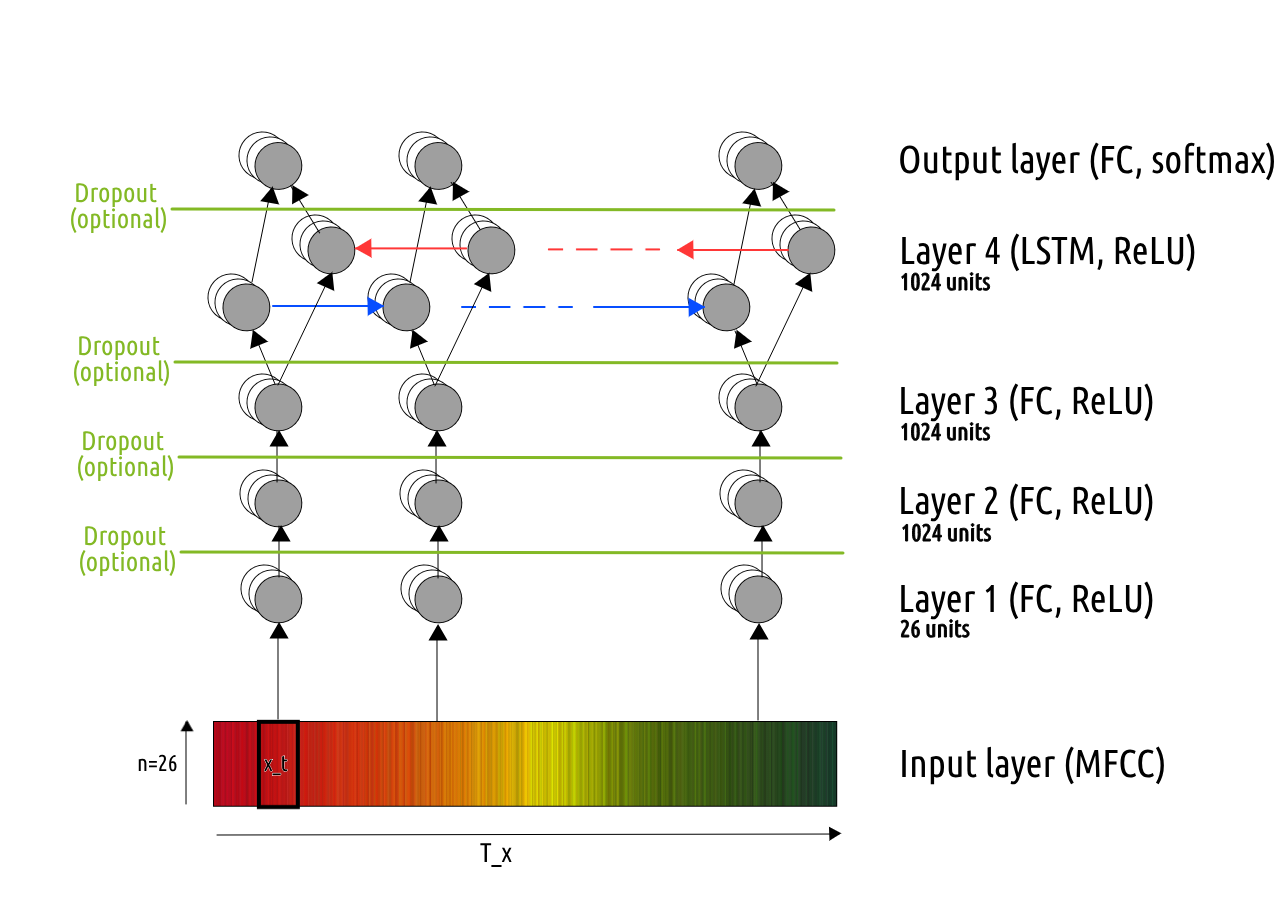
\includegraphics[width=\linewidth]{./img/model_architecture.png}
	\caption{Architecture of the simplified model. The cell type and the activation function is indicated in brackets for each layer (FC=Fully-Connected, ReLU=Rectified Linear Unit)}
	\label{model_architecture}
\end{figure}

\subsection{Summary}

This chapter described how a simplified variant of the \textit{DeepSpeech} model was derived from the Mozilla implementation. It also described the changes applied to the model from the IP8 project to help the model converge during training.
\clearpage

\section{Integrating a Language Model}\label{lm}

This chapter outlines the importance of \ac{LM}s for \ac{ASR}. It also describes how a \ac{LM} was integrated into the simplified \ac{DS} model as an attempt to improve the quality of the transcription.

\subsection{Measuring and improving the performance of a Speech-To-Text engine}

Although \ac{CTC} is the cost that is optimized during training, the usual metrics to evaluate an \ac{STT} system are \ac{WER} and \ac{LER}. These metrics corellate directly with the perceived quality of the system: Transcripts with a low \ac{WER} and/or \ac{LER} have a high similarity to the actual transcript and are considered accurate.

The \ac{LER} (sometimes also referred to as \textit{Levensthein Distance}) is defined as the mean normalized edit distance $ed(a, b)$ between two strings $a$ and $b$. It operates on character level by counting the number of insertions (\textit{I}), deletions (\textit{D}) and substitutions (\textit{S}) required to produce string $a$ from string $b$. String $a$ is the reference string, which in this project is the actual transcription of a speech segment (\textit{ground truth} or \textit{label}). String $b$ is a an inferred transcription produced by the simplified model (\textit{prediction}).  

The \ac{WER} builds upon the \ac{LER} and is therefore very similar. In contrast to \ac{LER} however, \ac{WER} operates on word level, i.e. it represents the number of words that need to be inserted, deleted or changed in a inferred transcription in order to arrive at the ground truth.

Both metrics can be normalized by dividing them by the length of the reference string i.e. the number of characters (\ac{LER}) resp. the number of words (\ac{WER}). If a single evaluation metric is required, the \ac{WER} is often the better choice because it is more related to the way humans assess the quality of a \ac{STT} engine: A transcription that might sound correct when read out loud, but is full of spelling mistakes, is not considered a good transcription. 

\subsection{Language Models in Speech Recognition}

\ac{LM}s model the probabilities of token sequences. Because a sentence is a sequence of word-tokens, a \ac{LM} can calculate its likelihood. Traditionally $n$-gram models (often simply referred to as \textit{$n$-grams}) have been used for this task. $n$-grams are overlapping tuples of words whose probability can be approximated by training on massive text corpora. A special token \code{<unk>} is used for unknown tokens that do not appear in the training corpus. Because of combinatorial explosion and the dynamic nature of human language, the computational power and storage which are needed to train higher-order models increases exponentially with the order $n$ of the model. Most models are trained on an order of $n=5$ or $n=6$. 

Because the context of $n$-gram models is determined by their order they are somewhat restricted in that they do not take into account words outside the context to assess the probability of a sentence. Although a lot of research has been made in the field of using \ac{NN} for language modelling (like for machine translation), $n$-grams \ac{LM} are still widely used and often a good choice for many tasks \parencite{slp3}. Because of their simplicity they are often faster to train and require significantly less training data than their neural counterparts.

\subsection{A simple spell checker}

The Mozilla implementation includes a $5$-gram \ac{LM}, which can be downloaded as a part of the pre-trained model from GitHub \footnote{\url{https://github.com/mozilla/DeepSpeech\#getting-the-pre-trained-model}}. This \ac{LM} was trained using \textit{KenLM}. The \ac{LM} is queried during training by decoding the numeric matrices produced by \ac{CTC} using \textit{Beam Search} or \textit{Best-Path} decoding. It uses a \textit{trie} and precompiled custom implementations of \textit{TensorFlow}-operations written in C  to maximize performance. 

As mentioned above, the \ac{LM} is deeply baked in with the training process of the Mozilla implementation, using its own hyperparameters. According to \cite{mozillajourney} this tight integration is the culmination of various attempts to integrate a \ac{LM} into the inference process. An early attempt used the \ac{LM} as some sort of spell checker that was able to correct minor orthographic errors. Rather than including the \ac{LM}-score during training, a spell-checker post-processes the inferences made by \ac{CTC} \textit{after} training. On one hand this deteriorates quality as has been shown by Mozilla, because no information from the \ac{LM} is used during training. On the other post-processing the inferences is simpler and reduces complexity. This supports the project premises of a preferably simple model. It can also be implemented with the standard tools provided by Keras and does not need to be precompiled into C. Post-processing the inferences with a spell checker was therefore the approach chosen for the simplified model.

The functionality of the spell checker can be summarized as follows (a more detailed and formal description can be found \hyperref[spellchecker]{in the appendix}): 

\begin{enumerate}
	\item Given an inference of space-separated word-tokens, process the words from left to right.
	\item For each word check if it is contained in the vocabulary of the \ac{LM}. 
	\begin{enumerate}
		\item If that is the case, continue with the next word. 
		\item If not, create a list of variations with edit distance 1 and keep only those variations that appear in the vocabulary. Each of these variations is a possible continuation that can be scored by the \ac{LM}. 
	\end{enumerate}
	\item If none of the variations appear in the vocabulary, create another list of variations with edit distance 2 to the original word. This list can be created recursively from the (complete) list of variations with edit distance 2. Again keep only those variations that appear in the vocabulary.	
	\item If none of the variations of the word with edit distance 2 are found in the vocabulary, use the original word as fallback. This can happen if the word is just gibberish or if the word is an actual valid word which does not appear in the training corpus for the \ac{LM} and has therefore never been seen before. Note that in this step the word must not be substituted by the \code{<unk>} token because it may still be a valid word. Furthermore, replacing the word with the \code{<unk>} token can have a contrary effect on the alignment, because this token will most likely never appear in a valid transcript. 
\end{enumerate}

Above steps are repeated until the whole sentence is processed. For each word this yields a cascade of possible combinations. Each of these combinations can be scored by the \ac{LM} as the sentence is being processed whereas only the $b$ most likely prefixes are kept at each step (beam search). For this project, a beam width of $b = 1.024$ was used. Figure \ref{spell-checker} illustrates how the spell-checker works.

\begin{figure}
	
\includegraphics[width=\linewidth]{./img/placeholder.png}
	\caption{Example of how the spell checker works}
	\label{spell-checker}
\end{figure}

A spell checker in combination with a \ac{LM} can help inferring orthographically correct words from sequences of characters inferred by \ac{CTC} and hence decrease the \ac{WER}. Therefore, by using a \ac{LM} the quality of transcriptions can improve considerably. Table \ref{ler_wer_example} illustrates this with an example.

\begin{table}[!htbp]
	\centering
	\begin{tabular}{llrrrr}
		\hline
		\thead{} &  & \thead{\ac{LER}} & \thead{\ac{LER}\\(norm.)} & \thead{\ac{WER}} & \thead{\ac{WER}\\(norm.)} \\
		\hline
		ground truth & i put the vice president in charge of mission control & $0$ & $0.00$ & $0$ & $0.00$ \\ 
		\hline
		before spell-checking & ii put he bice president in charge mission control & $6$ & $0.11$ & $4$ & $0.40$ \\ 
		\hline
		after spell-checking & i put the vice president in charge mission control & $3$ & $0.06$ & $1$ & $0.10$ \\
		\hline
	\end{tabular}
	\caption{Example for how a Spell-Checker (SC) can help improve the quality of an inferred transcription by changing characters and words. Audio and ground truth were taken from the \textit{ReadyLingua} corpus and the inference was made with the pre-trained \textit{DeepSpeech} model.}
	\label{ler_wer_example}
\end{table}

\subsubsection{Reducing the vocabulary size}

The \ac{LM} from Mozilla was trained on texts from the \textit{LibriSpeech} corpus\footnote{\url{http://www.openslr.org/11}}. Apart from lowercasing, the texts were not normalized or preprocessed. The resulting vocabulary is therefore very big and contains $973.673$ unique words. Because no further preprocessing was done, it also contains some exotic words like \textit{"zzzz"} and probably also misspelled words that happen to appear in the corpus. To train the \ac{LM}, $n$-grams of order 4 and 5 were pruned with a threshold value of 1, meaning only 4- and 5-grams with a minimum count of 2 and higher are estimated\footnote{see \url{https://github.com/mozilla/DeepSpeech/tree/master/data/lm}}. Because most spelling errors are probably unique within the training corpus, 4- or 5-grams containing an invalid word are unique too and most likely filtered out with pruning. 

Above procedure might work well to estimate the likelihood of a sentence. For a simple spell checker however, such a big vocabulary might be counter-productive because it lowers the probability that an obviously wrong word is corrected because for some reason it found its way into the vocabulary. Vice versa a very large vocabulary raises the probability that a random-looking sequence of characters is wrongfully exchanged with a (valid or invalid) word from the vocabulary. To prevent this, the original vocabulary was reduced into three vocabularies containing the $40.000$, $80.000$ and $160.000$ most frequent words from the corpus each. These words make up $98.42\%$, $99.29\%$ and $99.69\%$ of the corpus.

To create the vocabularies, a list of unique words and their frequency was created from the corpus and sorted by frequency in descending order. Naturally, stop words like \textit{the}, \textit{and} or \textit{of} appear at the top of the list. The first $40.000$, $80.000$ resp. $160.000$ words from this list were stored as the truncated vocabularies, the rest was discarded. Note that truncating the vocabulary only affects the way words are exchanged by the spell checker during post-processing, not how the likelihood of a post-processed sentence is estimated by the \ac{LM}.

\subsection{Further thoughts and considerations}

The spell checker in this project uses the vocabulary with $80.000$ words. This value was arbitrarily chosen and some unsystematic experiments were made to analyze the correctional capabilities of the spell checker. Because of time constraints and because it was unclear whether the spell checker would help improving the transcriptions in the first place, other vocabulary sizes were not evaluated. Further work may however try to find out an optimal vocabulary size for each language.

\subsection{Summary}

This chapter described how the $5$-gram \ac{LM} from the Mozilla implementation of \textit{DeepSpeech} was used to implement a rudimentary spell checker. This spell checker uses a vocabulary of the $80.000$ most frequent words from the corpus the \ac{LM} was trained on. It repeatedly swaps invalid words from an inferred transcript with valid words from the vocabulary and calculates the likelihood of various combinations of word sequences.
\clearpage

\section{Plotting a learning curve}

This section describes how training progress was monitored by plotting a learning curve.

\subsection{Previous corpora and their problems}

The following two corpora were available for training from the IP8 project.

\begin{itemize}
	\item \textbf{\ac{LS}}: This corpus was created as an artifact of the IP8 project using raw data from OpenSLR. The raw is publicly available and can be downloaded\footnote{\url{http://www.openslr.org/12/}}. It consists of a number of audio files which were \textit{partially} transcribed, i.e. there are parts in the audio for which the corresponding transcript is not exactly known (the audio contains \textit{gaps}). The individual samples were obtained by exploiting metadata that was included in the download. The metadata includes a split into a training set (containing approximately 96\% of the samples) and a validation resp. test set (each containing approximately 3\% of the samples). The split was done manually into disjoint subset, i.e. ensuring each speaker was only included in one set. Additionally, other features like gender or accent were observed to achieve a similar distribution for each set. To leverage the efforts made by \textit{OpenSLR}, this split was not changed.
	\item \textbf{\ac{RL}}: This corpus was created from raw data provided by \textit{ReadyLingua}. This data is proprietary and contains recordings in several languages which were manually aligned with their transcript. In contrast to the \ac{LS} corpus, the raw data is fully aligned, i.e. there are no gaps in the audio. However, the metadata does not comprise a split into training-, validation- and test-set. Since the raw data contained recordings and transcripts in more than one language, separate splits were made for each language preserving a ratio of approximately 80/10/10\% (relating to the total length of all recordings within each subset). Efforts were made to prevent samples from the same recording being assigned to different subsets. Other features were not observed, meaning the split into train/validation/test-set was done less carefully than in the \ac{LS} corpus.
\end{itemize}

The model in the IP8 project was supposed to be trained on the \ac{LS} corpus, because this corpus is much larger than the \ac{RL} corpus. In the course of the project it became clear however that training on all samples from this corpus was not feasible within project time because training time would have taken more than two months. It also turned out that the \ac{LS} corpus was probably less useful than initially assumed because the average sample length was much longer than the samples in the \ac{RL} corpus. This made training even harder because convergence is much slower when training on long sequences. The \ac{RL} corpus on the other hand consisted of shorter samples, but the total length of all samples was only a few hours compared to the 1000+ hours in the \ac{LS} corpus.

\subsection{The \textit{CommonVoice} Corpus}

Because of the aforementioned problems a new corpus was needed which combined the best of both worlds:

\begin{itemize}
	\item it should contain a reasonable amount of speech samples to facilitate training an ASR model
	\item the average sample length should be short enough for the model to learn quickly.
\end{itemize}

The \ac{CV}\footnote{\url{https://voice.mozilla.org/en/data}} corpus is maintained and used actively by the Mozilla Foundation and exhibits both of these properties. This corpus is also used to train the Mozilla implementation of \textit{DeepSpeech}. Datasets for various languages are being prepared and verified, each one containing speech samples of different contributors from all over the world. At the time of this writing, only the English dataset was available, but datasets for other languages will become publicly available at some time in the future. The English dataset comes pre-divided into training-, validation- and test-set of similar scale like the \ac{LS} corpus. Each set consists of one audio file per sample and a CSV file containing the transcriptions for each sample.

The simplified model in this project was trained on the training-set of the \ac{CV} corpus. Although still smaller than than the \ac{LS} corpus, the total length of all validated samples that can be used for training\footnote{CSV file: \code{cv-valid-train.csv}} is much larger than the \ac{RL} corpus while providing samples of similar length at the same time. Table \ref{corpora_stats} shows some statistics about the corpora described above.

\begin{table}[!htbp]
	\centering
	\begin{tabular}[t]{llrrrrr}
		\toprule
		\thead{Corpus} & \thead{Language} & \thead{total audio length} & train/dev/test & \thead{\# samples} & \thead{Ø sample\\length (s)} & \thead{Ø transcript\\length (chars)} \\
		\midrule
 		\ac{LS} & English & $24 days, 7:13:18$ & $93.51/3.32/3.16\%$ & $166,510$ & $12.60$ & $183.84$ \\ 
		\ac{RL} & English & $5:38:39$ & $80.39/10.13/9.48\%$ & $6,334$ & $3.20$ & $51.81$ \\ 		
		\ac{RL} & German & $1:58:30$ & $81.14/10.26/8.60\%$ & $2,397$ & $2.89$ & $45.55$ \\ 		
		\ac{CV} & English & $10 days, 1:02:53$ & $96.04/1.99/1.98\%$ & $201,252$ & $4.31$ & $48.07$ \\ 
		\bottomrule
	\end{tabular}
	\caption{Statistics about corpora that were available for training.}
	\label{corpora_stats}
\end{table}

\subsection{Plotting the learning curve}

The time needed to train an \ac{ASR} model on all samples of the \ac{CV} corpus is still too long for the available project time. We can however still get an estimate of the learning progress by plotting a \textit{learning curve}. For this, exponentially increasing amounts of training data (1, 10, 100 and 1,000 minutes of transcribed audio) were used. Training was done making 30 full passes over the training set (\textit{epochs}). The training samples were processed in batches of 16 samples each. They were sorted by the length of their audio signal and then zero-padded\footnote{sorting the samples was done to have sequences of similar length in each batch and thus reduce padding}, yielding samples of the same length in each batch\footnote{note that the length of the samples could still vary between batches}. 

After each epoch, the progress was monitored by inferring the transcriptions for previously unseen samples from the validation set. The \ac{CTC}-loss for training and validation was plotted for each amount, yielding separate curves for the training- and the validation-loss. Comparing both curves allows for making statements about at what point the Neural Network starts to overfit.

Complementary to the \ac{CTC}-loss, the mean values for the \ac{LER} and \ac{WER} metric over all samples in the validation set was calculated after each epoch, yielding the curves for the \ac{LER} resp. \ac{WER}. Observing these plots can give some insight about how well the network performs on unseen examples.

Both loss and metrics were compared along two dimensions:

\begin{itemize}
	\item \textbf{The decoder dimension}, comparing the two distinct ways to decode a transcript from the probability distributions calculated by the model for each frame in the input signal
	\item \textbf{The LM dimension}, comparing inferences made with and without post-processing the decoded transcript with a spell-checker as described above
\end{itemize}

Both dimensions are described in more detail below.

\subsubsection{Decoder dimension}

In a nutshell, \ac{CTC} aligns the $T_y$ characters from a known transcription (\textit{label} or \textit{ground truth}) with the $T_x$ frames from the input audio signal during training. $T_x$ is typically much larger than $T_y$ and must not be shorter. The characters (\textit{tokens}) in the label must come from an alphabet of size $V$, which for English are the 26 lowercased ASCII characters $a..z$, the space character and the apostrophe (because this character is very common in contracted words like e.g. \textit{"don't"} or \textit{"isn't"}). Additionally, \ac{CTC} introduces a special token $\epsilon$, called the \textit{blank token}, which can be used to label unknown/silent frames or prevent collapsing (see below). Consequently, the number of characters in the alphabet used by the \ac{ASR} in this project to recognize English is $|V|=26+1+1+1=29$.

\ac{CTC} is \textit{alignment-free}, i.e. it does not require an alignment between the characters of a transcription and the frames of an audio signal. The only thing needed is the audio signal $X$ itself plus its ground truth $Y$. Each token in the ground truth can be aligned with any number of frames in the input signal. Vice versa, repeated sequences of the same characters can be collapsed, whereas the $\epsilon$ token acts as a boundary within sequences of a token to prevent collapsing into one, when there should be two (such as in \textit{f-f-o-o-$\epsilon$-o-o-o-o-d-d-d}, which should collapse to \textit{food} and not \textit{fod}). 

For each frame input signal \ac{CTC} calculates a probability distribution over the $|V|$ characters in the alphabet. This yields a $|V| \times T_x$ probability matrix for the input signal. Because $T_x \ggg T_y$, there is usually a vast amount of different valid alignments collapsing to the same ground truth. The probability of each valid alignment can now simply be calculated by traversing the probability matrix from left to right and multiplying the probabilities of each character. Because calculating the probability of each valid alignment individually would be too slow and identical prefixes between valid alignments yield identical probabilities, a dynamic programming approach is usually chosen to calculate the probabilities whereas the intermediate probability for each prefix is saved once computed.

The most probable alignment is calculated by marginalizing (i.e. summing up) over the probabilities of the individual valid alignments. This calculation yields the CTC loss as a sum of products, which is differentiable and can therefore be optimized.

After training, a model using \ac{CTC} will again output a $|V| \times T_x$ probability matrix for any previously unseen input. This matrix can be used to infer a transcription, a process also known as \textit{decoding}. The \ac{CTC} paper proposes two different decoding strategies that are applied before collapsing the characters \cite{ctc_paper}:

\begin{itemize}
	\item \textbf{Best-Path (a.k.a. \textit{greedy}) decoding}: This strategy only ever considers the most likely character at each time step. The transcription before collapsing will be a single path through the the probability matrix, whose probability will be the product of all elements along the path. This approach is easy to implement but does not take into account the fact that a single output can have many alignments, whose individual probability may be lower than the one found with this strategy.
	\item \textbf{Beam-Search decoding}: This strategy approximates the probability of the most probable transcription by following multiple paths simultaneously and only keeping the $B$ most probable paths at each time step. The beam width is a hyperparameter that can be increased to get a more accurate transcription in exchange for higher computational cost.
\end{itemize}

Beam-Search decoding is expected to perform better. For the sake of completeness, both decoding strategies were compared in this project. This will yield separate learning curves for the decoder dimension. For Beam-Search decoding, the Keras implementation was used, which proposes a default beam width of $B=100$. This value was not changed. 

\subsubsection{\ac{LM} dimension}

Using a \ac{LM} to post-process the inferred transcription with a rudimentary spell checker will not necessarily lead to more accurate transcription, especially if the edit distance between prediction and ground truth is large. Table \ref{lm_bad_example} contains an example where the use of a spell checker is disadvantageous to the quality of a transcription.

\begin{table}[!htbp]
	\centering
	\begin{tabular}{llr}
		\toprule
		 &  & \thead{\ac{LER}} \\
		\midrule
		\textbf{ground truth} & i want to wish you a very happy thanksgiving & \\ 
		\textbf{prediction before spell-checking} & oento wiceyouepery appy thangksive & 0.4318 \\ 
		\textbf{prediction after spell-checking} & onto wiceyouepery app thangksive & 0.4545 \\ 		
		\bottomrule
	\end{tabular}
	\caption{Example of a transcription whose \ac{LER} was increased when using a spell checker}
	\label{lm_bad_example}
\end{table}

%ground truth: i want to wish you a very happy thanksgiving	
%prediction: oento wiceyouepery appy thangksive (LER=0.431818181818182, WER=1)
%prediction (LM-corrected): onto wiceyouepery app thangksive	(LER=0.454545454545455	WER=1)

%\begin{figure}[h!]
%	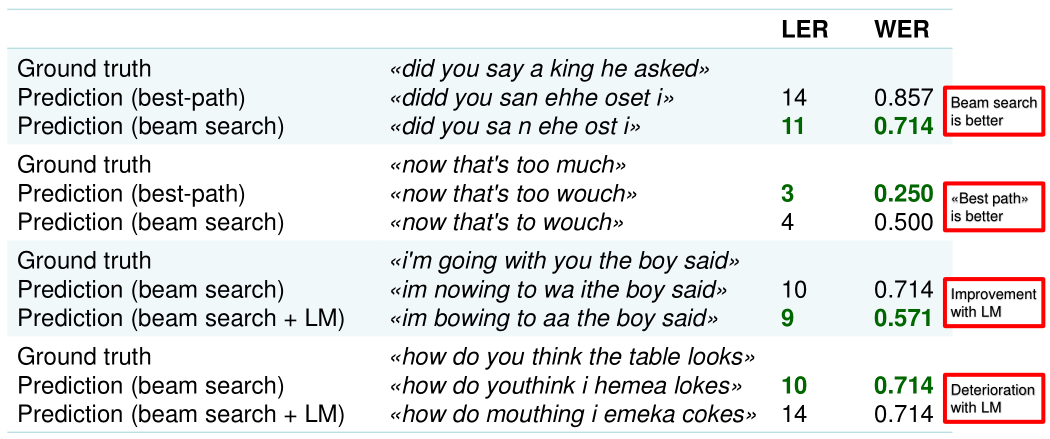
\includegraphics[width=\linewidth]{./img/lm_dimension_example.png}
%	\caption{Example of how a spell checker can improve or deteriorate the quality of a prediction.}
%	\label{lm_dimension_example}
%\end{figure}

In this example, \foreignquote{french}{\textit{oento}} was changed to \foreignquote{french}{\textit{onto}} because this was the most probable word with a maximum edit distance of 2 that was in the vocabulary. Similarly, \foreignquote{french}{\textit{appy}} was changed to \foreignquote{french}{\textit{app}}. This lead to a orthographically better sentence, but the \ac{LER} is higher than without spell-checking. 

It is generally expected that post-processing the inference as described above will lead to a lower \ac{WER}, supposed the \ac{LER} is already low enough, i.e. the prediction matches the ground truth already pretty well. If the \ac{LER} value is too high, the spell checker might try too hard to find a word from the vocabulary. This might result in a changed sentence consisting of real words but whose similarity to the ground truth is lower than before the changes. Post-processing might then be counter-productive. Therefore, separate learning curves were plotted for inference with and without post-processing (the \textit{\ac{LM} dimension})

\subsection{Results and interpretation}

Figure \ref{lc_loss_cv} shows the learning curve for the \ac{CTC}-loss. Obviously the training loss decreases steadily for all amounts of training data, converging to values between 30 (training on $1.000$ minutes) and 50 (training on 1 minute). Because the network does not generalize well when being trained on only 1 or 10 minutes of audio data, its predictions are somewhat random. This may be an explanation for the jagged curve of the validation plot (dashed lines) for these amounts of training data. When training on 100 minutes, the plot for the validation loss is smoother, but starts to increase between epoch 10 and 15, meaning the network starts to overfit after that point. When training on 1.000 minutes the validation loss does not decrease after epoch 14 anymore and plateaus at a value of about 90, meaning that any training will not contribute to a more generalizable network.

\begin{figure}[h!]
	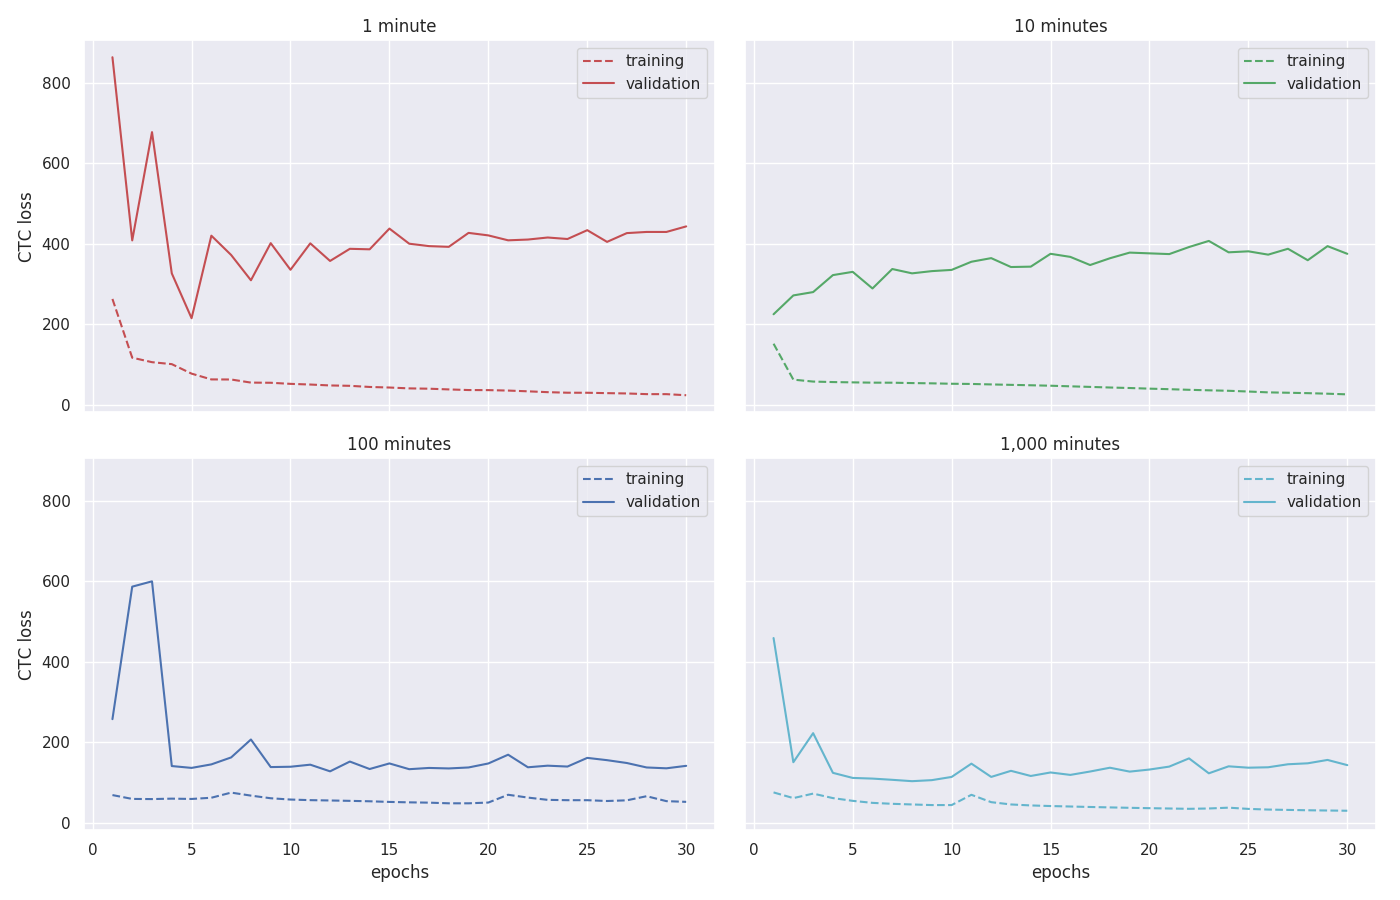
\includegraphics[width=\linewidth]{./img/lc_loss_cv.png}
	\caption{Learning curve for the CTC-loss while training on 1/10/100/1000 minutes of transcribed audio from the \ac{CV} corpus using the $5$-gram \ac{LM} provided by the Mozilla implementation of \textit{DeepSpeech}}
	\label{lc_loss_cv}
\end{figure}

Figure \ref{lc_ler_cv} shows how the average values of the \ac{LER} over all validation samples develops for the different amounts of training data. The plot on the left shows the results when using best-path decoding, the plot on the right for beam search decoding. The plots for all amounts of training data have been integrated in the same plot for the sake of a clearer representation. Both plots support the conclusions made for the CTC loss in that -- except when training on 1.000 minutes of audio -- the error rates do not decrease after epoch 15 anymore (in fact there is a slight increase). The plots for the \ac{LER} when training on 1.000 minutes are almost identical for both decoding strategies. Surprisingly, the \ac{LER} values continue to decline steadily, although only at a very slow rate, finishing with values of 0.54 (best-path decoding) resp. 0.52 (beam search decoding), meaning that the network got a bit more than half of the characters wrong, at the wrong position or entirely failed to predict them. The values when trying to correct the inferred transcriptions with a spell checker are slightly higher for both decoding strategies (0.55 and 0.53) meaning that post-processing did not help. This nourishes the assumption that a spell checker will probably only lower the \ac{WER} and only do so if the \ac{LER} is already low enough (see above).

\begin{figure}[h!]
	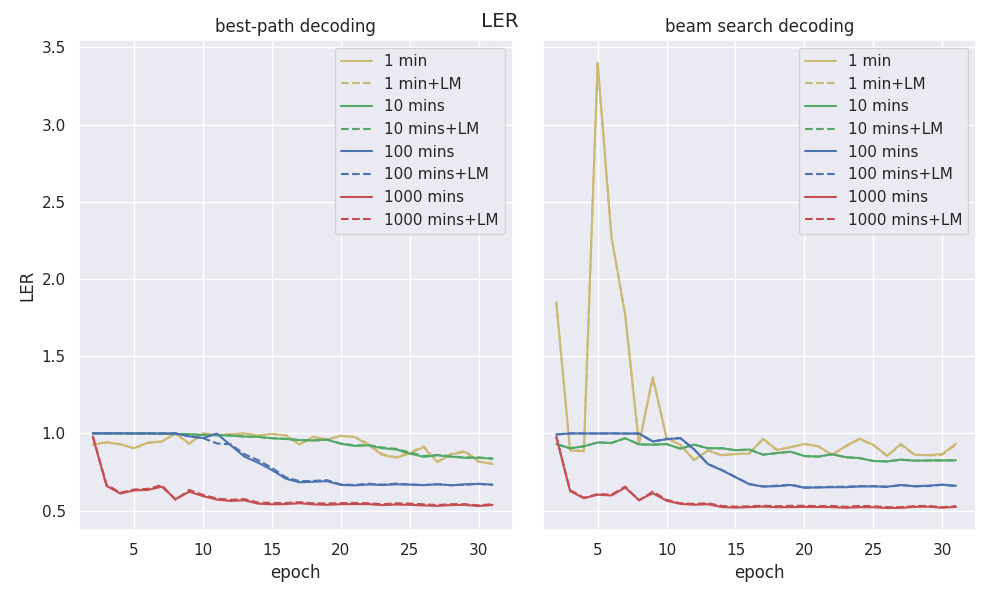
\includegraphics[width=\linewidth]{./img/lc_ler_cv.png}
	\caption{Learning curve for the \ac{LER} metric while training on 1/10/100/1000 minutes of transcribed audio from the \ac{CV} corpus with and without spelling correction with a \ac{LM}. For the lines where spelling was corrected, the $5$-gram \ac{LM} provided by the Mozilla implementation of \textit{DeepSpeech} was used.}
	\label{lc_ler_cv}
\end{figure}

Finally, figure \ref{lc_wer_cv} shows the development of the average \ac{WER} values over all validation samples. Not surprisingly, the plots oscillate around a value of 1, meaning the network did not get any of the words right. Only when training on 1.000 minutes, the network was able to achieve a value below 1, but is still way higher than the 0.0065 achieved by the Mozilla implementation of \textit{DeepSpeech}. It is noteworthy that the use of a spell checker marginally improves the results here.

\begin{figure}[h!]
	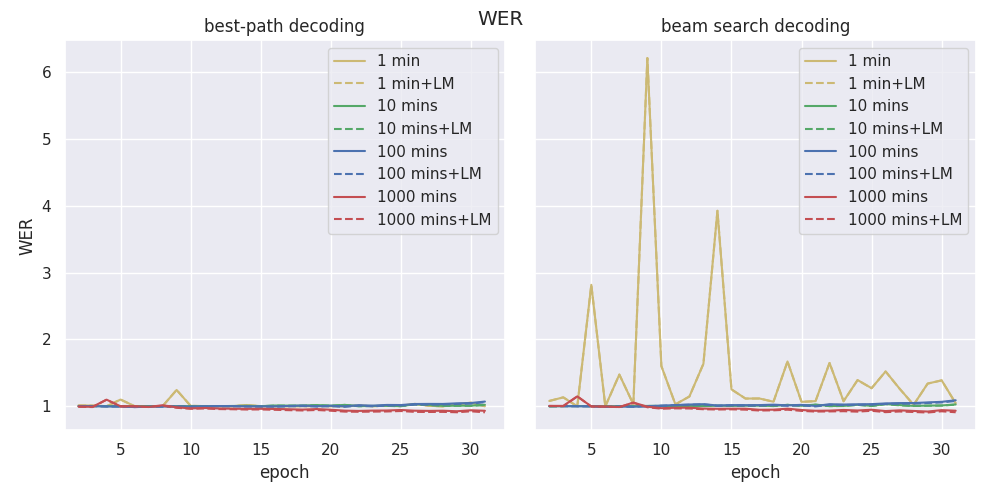
\includegraphics[width=\linewidth]{./img/lc_wer_cv.png}
	\caption{Learning curve for the \ac{WER} metric while training on 1/10/100/1000 minutes of transcribed audio from the \ac{CV} corpus with and without spelling correction with a \ac{LM}. For the lines where spelling was corrected, the $5$-gram \ac{LM} provided by the Mozilla implementation of \textit{DeepSpeech} was used.}
	\label{lc_wer_cv}
\end{figure}

In summary it can be said that the lowest \ac{LER} rates can be achieved when training on $1.000$ minutes of audio, not using the spell-checker. Training can be stopped after about 15 epochs however, because the results on validation data does not improve from there on. The average \ac{LER} of $0.52$ suggests that the network predicts about half of the characters right. This yields transcriptions which -- although far from correct -- are recognizeable as human language. Sometimes the real transcript might be guessed, especially for shorter sentences. Table \ref{training_progress} shows an example for how the accuracy of the inferred transcript improves with additional training data.

\begin{table}[!htbp]
	\centering
	\begin{tabular}{llll}
		\toprule
		\thead{training data} & \thead{inferred transcript} & \thead{\ac{LER}} \\
		\midrule
		1 minute & w t e isi & $0.76$  \\ 	
		10 minutes & tiar n th i id & $0.71$  \\ 		
		100 minutes & ave gos goe ei & $0.52$  \\ 		
		1.000 minutes & i've got go fi ha & $0.33$  \\ 		
		\bottomrule
	\end{tabular}
	\caption{Example of how the quality for inferred transcripts improves with additional training data. The \ac{LER} values were calculated against the ground truth \foreignquote{french}{\textit{i've got to go to him}}}
	\label{training_progress}
\end{table}

\subsection{Regularization}
As an attempt to prevent overfitting (or at least postpone it to later epochs), the network has been regularized by adding dropouts after each layer. The rate of each dropout has been set to 0.1, meaning a random 10\% of the unit weights in each layer will be zeroed out. Apart from adding dropouts no further changes were made to the simplified model.

The learning curve for the model with dropouts is similar to the one without dropouts, meaning its validation loss will plateau after about 15 epochs. To compare the simplified model with and without dropout, the average \ac{LER} on the \ac{CV} test-set was calculated with both decoding strategies. Table \ref{comparison_regularized_unregularized} shows the results of the comparison. The observations made for the spell checker also apply to the model with dropouts, meaning that the \ac{LER} rate is slightly better without spell-checking. The lowest average \ac{LER} rate (highlighted) was achieved using beam search and no spell checker. Although the difference is only marginal, the regularized model will be used for further evaluation.

\begin{table*}\centering
	\ra{1.3}
	\begin{tabular}{@{}rrrrcrrrcrrr@{}}\toprule
		& \multicolumn{2}{c}{Ø $LER$} \\
		\cmidrule{2-3}
		& not regularized & regularized\\ \midrule
		\textbf{best-path decoding}\\
		without spell-checker & 0.5359 & 0.5343 \\
		with spell-checker & 0.5475 & 0.5456 \\
		\textbf{beam search decoding}\\
		without spell-checker & 0.5146 & \cellcolor{green!25}0.5125 \\
		with spell-checker & 0.5256 & 0.5242 \\
		\bottomrule
	\end{tabular}
	\caption{Comparison of the simplified model with and without dropout regularization. The average \ac{LER} was calculated over all samples from the \ac{CV} test-set. The best value is highlighted.}
	\label{comparison_regularized_unregularized}
\end{table*}

%Figure \ref{lc_regularization_cv} show the difference between the original simplified model and the same model with dropouts added. Only the plots for training on $1.000$ are shown. Decoding was done using Beam-Search decoding. The plot on the left shows how the training/validation-loss develops for each model. The plot on the right shows how the average \ac{LER} on the validation set develops for each model.

%\begin{figure}[h!]
%	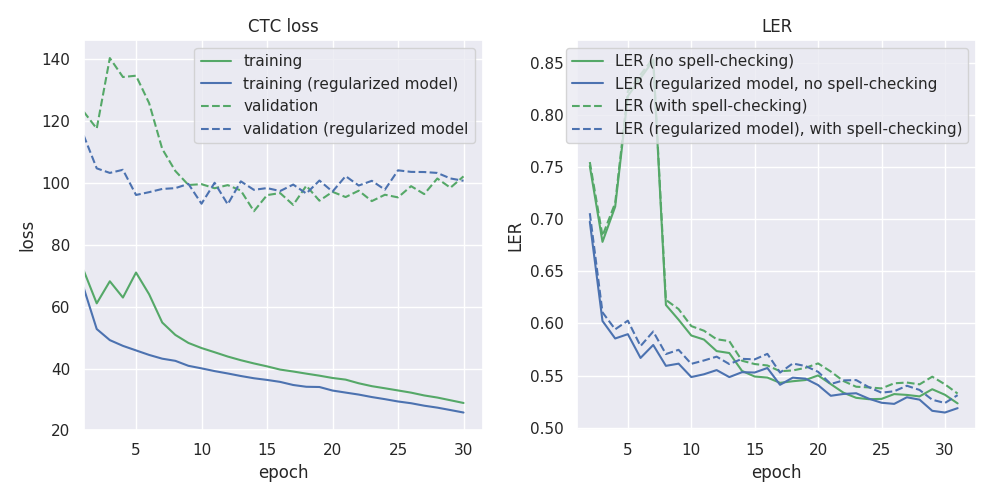
\includegraphics[width=\linewidth]{./img/lc_regularization_cv.png}
%	\caption{\ac{CTC}-loss and \ac{LER} values when training a simplified model with and without regularization. Apart from adding dropouts, no further changes were made to the original model. $1.000$ minutes of training data from the \ac{CV} corpus were used for training.}
%	\label{lc_regularization_cv}
%\end{figure}

\subsection{Final thoughts and considerations}

Above results were achieved with a spell checker using a vocabulary of 80.000 words and the 5-gram \ac{LM} from Mozilla. This did not help very much, but it might be possible that a different vocabulary size will produce better results. It is also possible that a different Optimizer, different dropout rates or integrating the \ac{LM} score into the cost function (like Mozilla did) will produce better results. Finally, it might be fruitful to train on smaller batches as it has been observed by \cite{batch_size_rnn} that with larger batches the quality of a model degrades. 

All these ideas produces many more combinations to try out, but preparing and running them is very time consuming. Because the \ac{LER} of about 0.5 (1.000 minutes, no spell checker) looks promising, I decided to leave it at this for the moment and see how far I get.

\subsubsection{Summary}

This chapter gave a quick introduction into how \ac{CTC} and its different decoding strategies work. It also gave an overview over the available corpora and showed how the training progress developed with varying amounts of training data, different decoding strategies and the use of a spell-checker. Post-processing the inferences with a spell-checker will not always lead to better transcripts. Training was done using samples from the \textit{CommonVoice} corpus. A regularized model was created by adding dropouts to the simplified model. The best results were obtained with the regularized model not using the spell-checker. When training this model on $1.000$ minutes of data the average \ac{LER} on test data is only slightly higher than $0.5$, meaning the model will get about 50\% of the characters in the transcript right. However it was also observed that both the regularized and unregularized model start to overfit after about 15 epochs.
\clearpage

\section{Measuring the performance of the pipeline}\label{e2e}

Above results reflect the performance of the \ac{ASR} stage alone. To get some insight about the quality of alignments produced by the whole pipeline, a simple web application was implemented that highlights the aligned parts of the transcript as the audio file is being played. This is very useful for an informal review, because the subjective quality of the alignments can be examined interactively. However, this method is not very systematic and infeasible for larger amounts of test data. To get a clearer sense of how well the pipeline performs, steps were taken to run large numbers of previously unseen samples through the pipeline and measure the quality of the final product (the alignments). This section describes how this was done.

\subsection{The quality of alignments}

Assessing the quality of alignments is not trivial because there is often no reference alignment to compare to. Even if there is one, assessing the quality of an alignment is somewhat subjective because a different alignment does not necessarily need to be worse or better. Objectively quantifying the quality of a result is difficult for an alignment pipeline because there is a a massive number of theoretically possible alignments for each audio/text combination. We can however derive a few objective criteria that make up a good alignment:

\begin{enumerate}
	\item The aligned partial transcripts should not overlap each other
	\item The alignments should neither start nor end within word boundaries
	\item The aligned partial transcripts should cover as much of the original transcript as possible	
	\item The aligned partial transcripts should be at the correct position, i.e. they should cover the actually spoken text
\end{enumerate}

The first criterion is enforced by changing the type of algorithm used for sequence alignment from a local to a global alignment algorithm. The \textit{Smith-Waterman} algorithm was used in the \ac{SA} stage in the IP8 project, which finds a local optimum for each transcript in isolation. The \ac{SA} stage in this project uses global sequence alignment (\textit{Needle-Wunsch} algorithm), which finds an optimal alignment for all partial transcrips at once. 

The second criterion is ensured by adjusting some of the alignments so that they fall exactly on word boundaries. This is done by moving the alignment boundaries produced by the \textit{Needle-Wunsch} algorithm to the left or right, depending on which one is closer. 

The remaining two criteria can be quantified with the following metrics (note the corellation\footnote{positive correlation: higher is better, negative correlation: lower is better}):

\begin{table}[!htbp]
	\centering
	\begin{tabular}{llll}
		\toprule
		\thead{criterion} & \thead{metric} & \thead{correlation} \\
		\midrule
		3 & \makecell[l]{length of text in ground truth that is not aligned\\vs. total length of the ground truth} & negative\\ \\ 	
		4 & \makecell[l]{average Levensthein similarity between the transcript\\and the text in the ground truth corresponding to its alignment} & positive \\ 
		\bottomrule
	\end{tabular}
	\caption{Metrics to evaluate the quality of alignments}
	\label{LM_evaluation}
\end{table}

Because the first metric measures how much of the target transcript is covered by the alignments, it is similar to the Recall metric ($R$) usually used for classification tasks, which measures how much of the target class was correctly classified. The second metric measures how well the produced results match up with the underlying parts of the transcript and is therefore similar to Precision ($P$), which the correctness of the classified results. Both metrics can hence be reduced to the \textit{F-score} ($F$):

\[ 
F = 2\cdot \frac{P\cdot R}{P+R}
 \]

\subsection{Test and results}

The pipeline was evaluated on the test set of the \textit{LibriSpeech} corpus containing 87 audio/text samples. Each sample was run through the pipeline twice, once using the simplified model and once using the pre-trained \textit{DeepSpeech} model (reference model) in its \ac{ASR} stage. Apart from the model used in the \ac{ASR} stage, all other stages in the pipeline were identical. For the simplified model, the dropout-regularized variant of the simplified architecture was used and trained on $1.000$ minutes of the original and synthesized data because this combination had the lowest average \ac{LER} on the validation data. Training was stopped early after 15 epochs to prevent overfitting.

The average values of $P$, $R$ and $F$ over all test samples was calculated for each pipeline as described above. Running the samples through both pipelines should help comparing the results produced by the first pipeline against a hypothetical optimum. Figure \ref{pipeline_boxplot_ls_en} shows for each model how the pipeline performs. 

Obviously the \textit{DeepSpeech} model provides very accurate transcripts which makes alignment easy in the following \ac{GSA} stage. Most values for $P$ lie therefore within a range of about $0.8$ and nearly $1.0$, except for a few outliers. The mean value is $0.865$. Because the simplified model was not trained for maximum speech recognition capabilities, the $P$-values are naturally lower and lie in a range of about $0.35$ and $0.55$ with a mean value of $0.435$. This is consistent with the average normalized \ac{LER} on the validation set of about $0.52$\footnote{the \textit{Levenshtein Similarity is the inverse of the normalized average \ac{LER}}}. 

In terms of coverage, both pipelines perform similarly well yielding mean $R$-values of $>0.999$. This is no surprise, because each alignment ends where the next one starts, thus there are no gaps in between unaligned parts can only occur at the very start or end of a transcript. 

The $F$-score for the pipeline using the \textit{DeepSpeech} model is quite compact with most values lying in the interval $[0.875, 0.975]$ (mean value: $0.926$), whereas the range is a bit bigger for the pipeline using the simplified model (mean value: $0.602$).

When testing the alignments with the web application, the subjective quality is very good for both pipeline variants. Only in a few cases the first or last word of an alignment should be assigned to the next resp. previous alignment.

\begin{figure}[h!]
	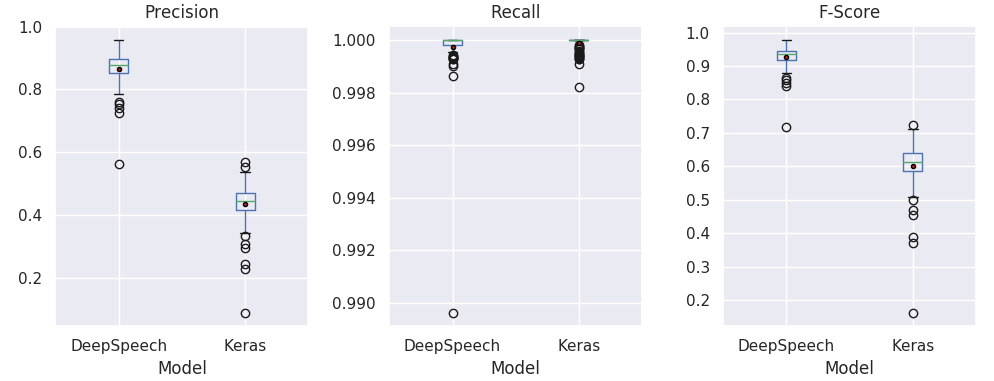
\includegraphics[width=\linewidth]{./img/boxplot_ls.png}
	\caption{Average values of $P$, $R$ and $F$ for a pipeline using the simplified \ac{STT} model compared to a pipeline using a state of the art model}. The \textit{DeepSpeech} model produces very accurate transcriptions and therefore very precise alignments ($P$ mean: $0.865$, median: $0.879$) and also a very high $F$-Score (mean: $0.926$, median: $0.935$). On the other hand, the simplified model produces only low-quality transcriptions, resulting in a lower Precision (mean: $0.435$, median: $0.443$). The $F$-Score is thus also lower (mean: $0.602$, median: $0.614$).
	\label{pipeline_boxplot_ls_en}
\end{figure}

Figure \ref{pipeline_scatterplot_ls_en} shows how the pipeline using the simplified model holds up against the pipeline using the reference model. It is evident that the \ac{LER} values between transcription and alignment are very low when using the reference model. When using the simplified model, the distribution of \ac{LER} values follows a similar pattern but is maybe a bit less compact on the y-axis and has a few more outliers. The mean average \ac{LER} value is $0.230$ when using the reference model and $0.982$ when using the simplified model. The length of the transcript resp. the recording does not seem to affect the performance of the alignment stage. Both pipeline variants have however one striking outlier belonging to a very long transcript ($>15.000$ characters), which was read by a fast-speaking woman. 

When comparing the similarity between the alignments made using the reference model and those made using the simplified model it is evident that the Levenshtein Similarity is very high with a mean value of $0.887$, regardless of the transcript length. This means the alignments are almost identical, only differring in single words sometimes at beginnings/endings of alignments being assigned to the previous/next alignment. There are a few cases where the similarity is lower (and the long transcript mentioned before, where the alignments are not similar at all). However it can be generally said that despite the simplified model producing low-quality transcriptions, the alignments do not differ much from the ones produced by a high-quality \ac{STT} engine.

\begin{figure}[h!]
	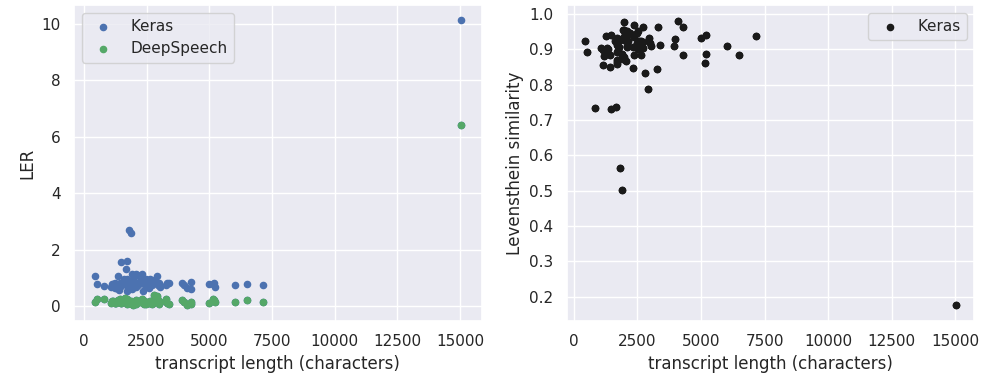
\includegraphics[width=\linewidth]{./img/scatterplot_ls.png}
	\caption{average \ac{LER} between transcript and alignment (left plot) and similarity between alignments made by using the pre-trained \textit{DeepSpeech} model and the simplified model (right plot). The average \ac{LER} values when using the simplified model (mean: $0.982$, median: $0.800$) follow the same pattern like when using the reference model (mean: $0.230$, median: $0.148$), but are generally higher due to the lower quality of the transcriptions. However, this does not seem to affect the alignments produced by the two pipelines. The average similarity between alignments produced by the pipeline using the simplified model are roughly the same like when using the reference model (mean: $0.887$, median: $0.909$).}
	\label{pipeline_scatterplot_ls_en}
\end{figure}

\subsection{Summary}

This chapter demonstrated how the quality of alignments produced by the pipeline was measured. Since this quality is subjective, the results of the pipeline using the simplified \ac{STT} model were compared to the results of the same pipeline using the pre-trained \textit{DeepSpeech} model as a reference model. It was observed that although the quality of transcriptions is notably lower for the former pipeline, the resulting alignments are very similar for both pipelines. This means the \ac{GSA} stage can handle transcripts of much lower quality and still produce a good alignment.
\clearpage

\section{Forced Alignment for other languages}

So far, only audio and transcripts in English were considered. A fully automated solution however should be able to align text and audio in any other language. Because of linguistic characteristics like sound patterns and morphology the results might vary a lot between languages when tested under identical circumstances. To get some intuition about the influence of language and whether above conclusions are transferable to other languages, the pipeline was evaluated on the German samples received from \textit{ReadyLingua}.

\subsection{Inferring German transcripts}

Enabling the pipeline to handle German samples means training a German \ac{ASR} as its core element. This requires minimal modifications to the network architecture, because German transcripts use a different alphabet. As mentioned before, the apostrophe is far less common in German than in English and was therefore dropped. On the other hand, umlauts are very common in German and were added to the 26 ASCII characters. Since the alphabet represents all possible labels, the output layer in the model needs to be changed to contain 31 units (one for each character in the alphabet, the three umlauts, space plus a blank token) instead of the 29 units used for English.

Training an \ac{ASR} model for German and plotting a learning curve also requires amounts of training data on a similar scale like the \ac{CV} corpus used for English. Since at the time of this writing, the \ac{CV} was still a work in progress, datasets for languages other than English were not available. High-Quality \ac{ASR} corpora are generally hard to find, especially considering the number of samples needed to train a \ac{RNN}. There are corpora for \ac{ASR} in German, but those are either not freely available or their quality is unknown. An extensive list of German corpora for various purposes can be found at the \ac{BAS}\footnote{\url{https://www.phonetik.uni-muenchen.de/Bas/BasKorporaeng.html}}, including exotic corpora like the \textit{ALC} corpus\footnote{\url{http://www.bas.uni-muenchen.de/forschung/Bas/BasALCeng.html}} containing recordings of intoxicated people. Some of the corpora on this list are free for scientific usage and have been used by \cite{budget} to train their German \ac{ASR} model with transfer-learning. However, not all of these corpora are targeted at \ac{ASR} and their quality is often unknown.

\subsection{Data augmentation}

Integrating new raw data means preprocessing the audio (e.g. resampling) and the text (e.g. normalization, tokenization) to make sure it exhibits the same properties as the other corpora and the data conforms to the target format. This step is usually very time consuming, often taking most of the project time. Because no ASR corpus for German was readily available, training was done on the data received from \textit{ReadyLingua} as a start. The alignment between audio and transcript in this corpus was done manually and is therefore very accurate. Audio and text were already preprocessed in the IP8 project and the metadata was processed and stored as a corpus. The individual training samples could therefore be transformed to the format expected by the Mozilla implementation of \textit{DeepSpeech} (and thus by the simplified model) with comparably little effort. Also, the samples exhibited similar properties (average audio and transcript length) like the \ac{CV} corpus (refer to table \ref{corpora_stats}). However, the total length of the samples in the training set was only about one and a half hours, which was much less than the 1000+ minutes in the \ac{CV} corpus and certainly not enough for the $1.000$ minutes needed to plot a learning curve like to the one made for English. 

An easy way to get more training data is augmenting existing data by synthesizing new data from it. This is particularly easy for audio data, which can be distorted in order to get new samples corresponding to the same transcript. The following distortions were applied in isolation to each sample in the training set:

\begin{itemize}
	\item \textbf{Shifting}: The frames in the input signal were zero-padded with samples corresponding to a random value between $0.5$ and $1.5$ seconds, shifting the signal to the right, i.e. starting the signal later. This resulted in one additional synthesized sample for each original sample. Shifting to the left was not done to prevent cropping parts of the speech signal.
	\item \textbf{Echo}: The presence of echo can be generated with the Pysndfx library\footnote{\url{https://github.com/carlthome/python-audio-effects}} using random values for delay and damping. This resulted in one additional sample.
	\item \textbf{Pitch}: The pitch of the signal was increased or decreased. Increasing and decreasing was done using two different random factors, resulting in two additional samples. This can be seen as a rudimentary way to simulate a female from a male speaker or vice versa.
	\item \textbf{Speed}: Faster or slower speaking rates can be simulated by "stretching" or "compressing" the signal while preserving the pitch. Similar to the change in pitch, two different random factors were use to change the tempo. This resulted in two additional samples.
	\item \textbf{Volume}: The loudness of the speaker was artificially reduced or increased by a random value within the range of $[-15..-5]$ resp. $[5..15]$ db. This resulted in two additional sample.
\end{itemize}

With above methods eight synthetisized samples can be created for each original sample from the corpus. It turned out however that this was still not enough to plot a learning curve. To augment the data to the 1.000 minutes needed, additional samples were created using random combinations of the distortions. The random parameters differed from the ones used before to prevent overfitting to the distortion. Table \ref{corpus_synth_stats} shows the corpus statistics before and after data augmentation.

\begin{table}[!htbp]
	\centering
	\begin{tabular}{lrrrr}
		\toprule
		\thead{} & \thead{total audio length} & \thead{\# samples} & \thead{Ø sample length (seconds)} \\
		\midrule
		before augmentation & $1:36:09$ & $1,700$ & $2.89$ \\ 		
		after augmentation & $16:40:00$ & $18,955$ & $3.16$ \\ 		
		\bottomrule
	\end{tabular}
	\caption{Comparison of \ac{RL} corpus before and after data augmentation (training set only)}
	\label{corpus_synth_stats}
\end{table}


\subsection{Creating a Language Model for German}

Since the \ac{ASR} stage in the pipeline uses a spell-checker querying a \ac{LM} to post-process the results a $5$-gram model similar to the one created by Mozilla needed to be trained first. The following sections require understanding some methods of $n$-grams like smoothing, discount and backoff. A short explanation of how $n$-grams work is given \hyperref[n-gram-summary]{in the appendix}.

\subsection{Creating a raw text corpus}

To train a $n$-gram model for German, a raw text corpus of German Wikipedia articles was used as corpus. Like the English $n$-gram from Mozilla KenLM \parencite{kenlm} was used to estimate the probabilities. The articles were pre-processed to meet the requirements of \textit{KenLM}. It was normalized as follows 

\begin{itemize}
	\item remove Wiki markup
	\item remove punctuation
	\item make everything lowercase
	\item \textbf{Unidecoding}: translate accentuated characters (like \code{è,é,ê}, etc.) and special characters (like the German \textit{ß}) to their most similar ASCII-equivalent (\code{e} resp. \code{ss}). This process helps accounting for ambiguous spelling variants of the same word and misspelled words. It also reduces the number of unique words by reducing different versions to a normalized variant. A special case are umlauts. Although also not part of the ASCII code set, they were kept as-is because they are very common in German.
	\item \textbf{Tokenization}: Because \textit{KenLM} expects the input as sentences (one sentence per line), the raw text was further tokenized into sentences and words using NLTK \parencite{nltk}. 
	\item \textbf{Numeric tokens}: Word tokens that are purely numeric (such as year numbers) are replaced with the special token \code{<num>}. Although such tokens occur frequently in the Wikipedia articles, they are unwanted in the corpus because they represent values and do not carry any semantic meaning. Because there is a infinite number of possible numeric tokens, they were all collapsed to the same normalized token.
\end{itemize}

The corpus was saved as text file containing one normalized sentence per line. The special tokens \code{<s>} and \code{</s>} are used to mark beginnings and endings of sentences as well as the \code{<unk>} token which is traditionally used to represent \ac{OOV} words. They are however not part of the corpus because they are added automatically by \textit{KenLM}.

The following lines are an excerpt of a article in the German Wikipedia along with its representation in the corpus.

\begin{displayquote}[German Wikipedia article about Speech Recognition\footnote{\url{https://de.wikipedia.org/wiki/Spracherkennung}}]
	Die Größe des Wörterbuchs hängt stark von der Sprache ab. Zum einen haben durchschnittliche deutschsprachige Sprecher mit circa 4000 Wörtern einen deutlich größeren Wortschatz als englischsprachige mit rund 800 Wörtern. Außerdem ergeben sich durch die Flexion in der deutschen Sprache in etwa zehnmal so viele Wortformen, wie in der englischen Sprache, wo nur viermal so viele Wortformen entstehen.
\end{displayquote}

\begin{lstlisting}[numbers=left, caption=Representation in corpus]
die grösse des wörterbuchs hängt stark von der sprache ab
zum einen haben durchschnittliche deutschsprachige sprecher mit circa <num> wörtern einen deutlich grösseren wortschatz als englischsprachige mit rund <num> wörtern
ausserdem ergeben sich durch die flexion in der deutschen sprache in etwa zehnmal so viele wortformen wie in der englischen sprache wo nur viermal so viele wortformen entstehen
\end{lstlisting}

Like for the English spell checker, three vocabularies containing the $40.000$, $80.000$ and $120.000$ most frequent words from the corpus was created. The words from these vocabularies make up $87.75\%$, $90.86\%$ resp. $93.36\%$ of the total number of words in the corpus. It is expected that the optimal number of words in the vocabulary is higher for German than for English. This is due to the fact that different flexions of the same word are very common in German due to grammatical conjugations (different forms for the same verb) and declinations (different cases for the same noun). Therefore German tends to apply a wider range of words and the size of vocabulary had to be increased. Handling the different flexions would require lemmatization and/or stemming the corpus in order to reduce them to a common base form. This has not been done for simplicity and time constraints. It is also doubtful whether this would actually help improving the quality of inferred transcripts, since humans do not speak in lemmata or stems.

\subsection{Training the \ac{LM}}

The final corpus contained data from 2,221,101 Wikipedia articles (42,229,452 sentences, 712,167,726 words, 8,341,157 unique words). This corpus was used to train a $5$-gram \ac{LM} using \textit{KenLM}. \textit{KenLM} uses \textit{Kneser-Ney Smoothing} and some optimization techniques called \textit{quantization} and \textit{pointer compression}. 

\subsubsection{Data structures}
$n$-grams can be represented with a prefix-tree structure (called \textit{Trie}) \footnote{note that \textit{KenLM} offers a so called \textit{PROBING} data structure, which is fundamentally a hash table combined with interpolation search, a more sophisticated variant of binary search, which allows for constant space complexity and linear time complexity. This does however not change the fact that $n$-grams can conceptually be thought as a tree of grams}, which allows for pruning. $n$-grams of order 2 and higher can be pruned by setting a threshold value for each order. $n$-grams whose frequency is below the threshold will be discarded. \textit{KenLM} does not support unigram pruning.

\subsubsection{Quantization}
To save memory, the amount of bits used to store the non-negative log-probabilities can be reduced with the parameter $q$ to as little as $q = 2$ bits at the expense of accuracy. This reduction yields $2^q -1$ possible bins. The value of each bin is calculated by equally distributing the probabilities over these bins and computing the average. Note that the quantization is done separately for each order and unigram probabilities are not quantized.

\subsubsection{Pointer Compression}
To use memory even more efficiently, the pointers which are used to store $n$-grams and their probabilities can be compressed. Such pointers are used to represent e.g. word IDs (for $q$-grams) and are stored as sorted integer-arrays. Additionally, These integers can be compressed using a lossless technique from \cite{raj_lossless} by removing leading bits from the pointers and store them implicitly into a table of offsets. The parameter $a$ controls the maximum number of bits to remove. There is a time-space trade-off meaning that a higher value of $a$ will lead to a smaller memory footprint at the cost of a slower training time.

\subsubsection{Building the model}

The a $5$-gram \ac{LM} was trained on the German Wikipedia corpus using  using the Trie data structure and the same parameters like the model downloaded from \textit{DeepSpeech} ($q=8$ and $a=255$). Like the \textit{DeepSpeech} model $4$- and $5$-grams were pruned by setting a minimum frequency of $1$.

%Pruning 1-grams would help getting rid of obvious spelling mistakes and very rare tokens that only appear in very special contexts. Unfortunately, \textit{KenLM} does not support pruning unigrams, only higher-order $n$-grams. Therefore the vocabulary used for training was limited to the 500,000 most frequent words not containing numbers with a minimum length of 2 characters \footnote{this constraint was imposed because NLTK did sometimes not tokenize abbreviations like \textit{z.B.} correctly, which resulting in two separate tokens \code{z} and \code{b}}. Note that this amount is about the same what was used in the \textit{DeepSpeech} paper \parencite{deepspeech} but more than the $250.000$ words used for the English spell checker. 

%The 500k most frequent words in the vocabulary make up 96.42\% of the whole corpus. The most frequent word in the vocabulary is the \code{<num>} token (29,659,021 counts). The least frequent word is \textit{Flachmeeres} (31 counts), which is actually a derivate of another German word \textit{Flachmeer}, which also appears in the vocabulary (109 counts) and which is an example of above mentioned flexion. 

%By limiting the vocabulary to the 500k most frequent words, the unigrams in the KenLM were artificially pruned. The number of unigrams was therefore 500,003 (one unigram for each word in the vocabulary plus one each for the \code{<s>}, \code{</s>} and \code{<unk>} tokens). The $n$-grams used to train the \ac{LM} have been pruned by setting the minimal threshold for $n$-Grams of any order ($n \in 1..4$) to 40. This is the value that Google used (reference from Jurafsky). Pruning unigrams helped getting rid of obvious spelling mistakes and very rare tokens that only appear in very special contexts (like the tokens \textit{aaaaa} or \textit{zzyzzyxx}) (EDIT: Pruning unigrams is not supported by KenLM, but the vocabulary can be limited). Such words are mostly not no real German words and should therefore not be trained on. Pruning higher-order $n$-grams was done to increase performance (both in space and time).

\subsection{Evaluating the \ac{LM}}

Literature suggests two methods to evaluate a \ac{LM}: Extrinsic and intrinsic evaluation.

\subsubsection{Extrinsic and intrinsic evaluation}

The best way to evaluate a \ac{LM}is to embed it in an application and measure how much the application improves \parencite{slp3}. This is called \textit{extrinsic evaluation} and has been done by comparing the learning curves with and without using a \ac{LM}. However, to measure the performance of a \ac{LM} independently (\textit{intrinsic evaluation}) one would have to provide a test set containing unseen sentences an assess the scores of the \ac{LM} on their $n$-grams. The results can then be compared to a reference \ac{LM}: Whatever model produces higher probabilities (or lower perplexity) to the $n$-grams in the test set is deemed to perform better. However, models can only be compared if they use the same vocabulary and always encode characteristics of the training corpus \parencite{slp3}. Since the sentences in a corpus of legal documents use different structures and word distributions than a corpus of children's books, two models trained on these corpora will not be comparable. Evaluating the created German Wikipedia corpus intrinsically would therefore require training a reference model on the same corpus, which can become very time consuming.

\subsubsection{Evaluation of KenLM}

\textit{KenLM} has been extensively compared to other \ac{LM} implementations like \ac{SRILM} both in terms of speed and accuracy. It has been found to be both faster and more memory efficient \parencite{kenlm} than the fastest alternative. Its low memory profile makes it runnable on a single machine, while other algorithms like \textit{MapReduce} target clusters \parencite{kenlm_estimation}. The highly optimized performance was a big advantage especially for this project because it enabled testing the model on a local machine. The probabilistic performance of \textit{KenLM} has been evaluated by training a $5$-gram model on a 126 billion token corpus (393 million unique words) \parencite{kenlm_estimation}. This model was embedded in some Machine Translation systems (Czech-English, French-English and Spanish-English) . Evaluation was done by calculating the BLEU score and comparing it to embeddings of other \ac{LM}. \textit{KenLM} placed first in all submissions.

\subsubsection{Evaluation of the German Wikipedia \ac{LM}}

Because of time constraints and because \textit{KenLM} has already been extensively evaluated on English I resigned from evaluating my German \ac{LM} intrinsically, even though the corpus used for training is not as big as the one used in \cite{kenlm_estimation}. \textit{KenLM} is to date widely recognized as the best performing \ac{LM} available, which is also emphasized by the usage of a \textit{KenLM} model in the Mozilla implementation of \textit{DeepSpeech}.

To still get an intuition about how well the model performs, two different experiments were made:

\begin{itemize}
	\item \textbf{Experiment 1}: The probability calculated for valid German sentences was compared against variants of the same sentences with the words in randomized order.
	\item \textbf{Experiment 2}: The \ac{LM} was used together with its vocabulary to build a simple word predictor.
\end{itemize}

Both experiments are explained in more depth below.

\subsubsection{Evaluation 1: Comparing scores of randomized sentences}

The first experiment tests the validity of the probabilities (\textit{scores}) calculated by the \ac{LM}. For this, an arbitrary choice of 5 valid sentences in German was used. To ensure the sentences could not have been seen during training, the following 5 sentences were taken from a newspaper printed after the creation of the Wikipedia dump:

\begin{lstlisting}[numbers=left, caption=Representation in corpus]
Seine Pressebeauftragte ist ratlos.
Fünf Minuten später steht er im Eingang des Kulturcafés an der Zürcher Europaallee.
Den Leuten wird bewusst, dass das System des Neoliberalismus nicht länger tragfähig ist.
Doch daneben gibt es die beeindruckende Zahl von 30'000 Bienenarten, die man unter dem Begriff «Wildbienen» zusammenfasst.
Bereits 1964 plante die US-Airline Pan American touristische Weltraumflüge für das Jahr 2000.
\end{lstlisting}

All sentences have been normalized the same way sentences were preprocessed for training. For each of them the score was calculated. Then the words were shuffled and the score was calculated again. A good \ac{LM} should calculate a (much) higher probability for the original sentence, because the shuffled sentence is most likely just gibberish.  Table \ref{LM_evaluation} shows the results of the comparison. It is evident that the probabilities for the shuffled sentences are much lower than for the sentences where the words appear in the correct order. The probabilities calculated by the \ac{LM} are therefore deemed valid.

\begin{table}[!htbp]
	\centering
	\begin{tabular}{lrlr}
		\toprule
		\thead{original sentence (normalized)} & \thead{score} & \thead{permuation} & \thead{score} \\
		\midrule
		\makecell[l]{seine pressebeauftragte\\ist ratlos} & -17.58 & \makecell[l]{ist ratlos\\pressebeauftragte seine} & -21.52 \\
		\makecell[l]{fünf minuten später steht\\er im eingang des kulturcafes\\an der zürcher europaallee} & -40.23 & \makecell[l]{des er minuten zürcher kulturcafes\\steht europaallee eingang\\fünf im später an der} & -57.69 \\
		\makecell[l]{den leuten wird bewusst\\dass das system des \\ neoliberalismus nicht\\länger tragfähig ist} & -35.52 & \makecell[l]{system nicht das ist\\dass leuten tragfähig des\\neoliberalismus den\\bewusst länger wird} & -51.27 \\
		\makecell[l]{doch daneben gibt es die\\beeindruckende zahl von \code{<num>}\\bienenarten die man unter dem\\begriff wildbienen zusammenfasst} & -48.36 & \makecell[l]{dem gibt wildbienen zahl\\beeindruckende doch man\\zusammenfasst es daneben bienenarten\\von die unter die \code{<num>} begriff} & -75.95 \\
		\makecell[l]{bereits \code{<num>} plante\\die usairline pan american\\touristische weltraumflüge\\für das jahr \code{<num>}} & -58.04 & \makecell[l]{plante touristische für\\jahr pan american das\\bereits usairline \code{<num>}\\\code{<num>} weltraumflüge die} & -64.02 \\
		\bottomrule
	\end{tabular}
	\caption{Comparison of log10-probabilities calculated for news sentences and a permutation of their words}
	\label{LM_evaluation}
\end{table}

\subsubsection{Experiment 2: Word predictor}

The second experiment tests whether the trained \ac{LM} is able to continue a sentence given its beginning. For this each word from the vocabulary is appended and the score of the resulting stumps is calculated. The most likely continuation can be estimated by sorting the resulting list in descending order (the probabilities are $\log_10$-based, i.e. negative) and taking the first element. This behavior can be applied iteratively to construct a sentence from a stump. For this experiment a sentence was started with the stump \foreignquote*{french}{\textit{Ein 2007 erschienenes}}. Afterwards a word from the five most probable continuations was appended. The extended stump was then again fed into the \ac{LM}. This process was repeated until some kind of sentence ending was encountered. Each extended stump was preprocessed the same way the sentences were preprocessed for training (lowercasing, replacing numbers with \code{<num>}, etc.). Figure \ref{word_predictor} shows the path taken through the predictions. Note that the predictions for the second and third word of the stump after typing the first word are shown in grey for illustrative purposes, although they were not considered for continuation.

\begin{figure}[h!]
	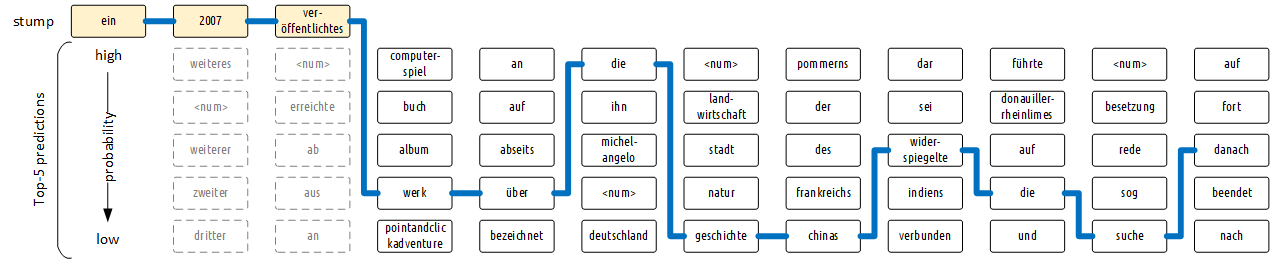
\includegraphics[width=\linewidth]{./img/word_predictor.png}
	\caption{Word predictions of the trained 5-gram model for continuations of the stump \foreignquote*{french}{\textit{Ein 2007 erschienenes ...}}. The blue path represents a grammatically valid German sentence.}
	\label{word_predictor}
\end{figure}

Although prediction was slow we can observe that the words suggested by the \ac{LM} are generally grammatically correct continuations and often make sense, although the probability for some of the predicted words (like \textit{Michelangelo}) is sometimes unexplicably high. Nevertheless it was possible to create a valid German sentence from the stump using only the suggested words. The \ac{LM} even seems to have captured some notion about grammatical concepts like German cases (e.g. that \foreignquote{french}{\textit{die Geschichte Chinas}} is more likely than \foreignquote{french}{\textit{die Geschichte China}}). On the other hand we can observe that the meaningfulness of the suggestions decreases with the progress because some long-distance relationships between words are lost for small values of $n$.

\subsection{\ac{STT} model performance}

The observations made when training the simplified Keras model on German audio data are similar to the ones made when training on English data in that the spell-checker will not help and the CTC validation loss will decrease until epoch 15 and then plateau or increase slightly.

When evaluating the \ac{LER} metric on the test set, the best performance was achieved with a regularized model that was trained on 1.000 minutes of audio, including synthesized samples. The average \ac{LER} value was then $0.4918$, which is even better than the $0.5125$ achieved when training on English samples from the \ac{LS} corpus. This result has to be taken with a pinch of salt though, because the test data in the \ac{RL} corpus is not as extensive as the one from the \ac{LS} corpus and it has also not been extracted with the same diligence. 

The effect of regularisation and/or use of synthesized training data can be visualized. Figure \ref{regularization_synthetisation} shows both measures in isolation and in combination. From the plot on the left it becomes evident that transcripts inferred by a regularized model will generally have a lower \ac{LER} than without regularisation. The plot in the middle shows how the use of synthesized training data has a smoothing effect on the curve of the \ac{LER}. Finally, the plot on the right shows the progress of the average \ac{LER} values when combining both measures, i.e. training a regularized model with training data including synthesized samples. The effect is bot a smoother curve and mostly lower \ac{LER} rates, although there is an awkward spike between epoch 15 and 20.

\begin{figure}[h!]
	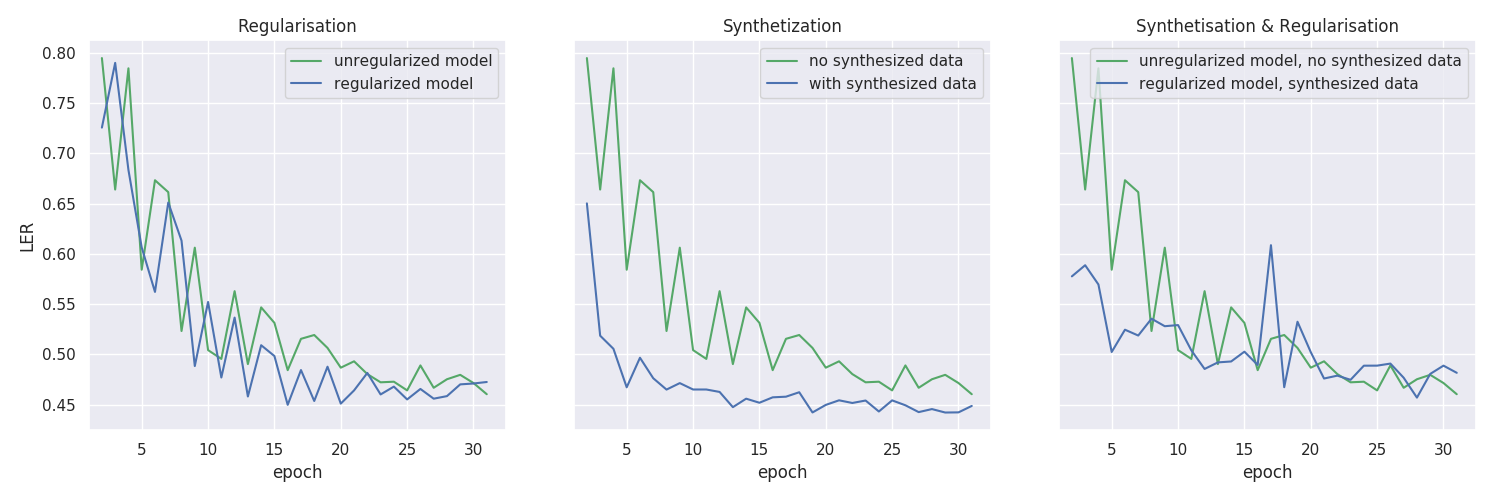
\includegraphics[width=\linewidth]{./img/regularization_synthetisation.png}
	\caption{Impact of regularization and/or synthetisation on the progress of average \ac{LER} values. Regularization alone (left) will lead to lower \ac{LER} rates. Synthesized training data (middle) will lead to a smoother curve and lower \ac{LER} rates. Both measures combined will also combine their effects, although the trend is less obvious.}
	\label{regularization_synthetisation}
\end{figure}

\subsection{Pipeline performance}

Because the regularized model trained with synthesized data has both the lowest \ac{LER} rates and a smoother curve, this model is used in the \ac{ASR} stage of the pipeline when aligning German samples. The pipeline can then be evaluated like it was evaluated for English samples. However, while for English samples the Mozilla implementation of \textit{DeepSpeech} could be used as a reference model, such a reference model is not available for German\footnote{except proprietary \ac{STT} engines like \textit{Google Cloud Speech}, which are only available online} because the \textit{CommonVoice} German dataset is not mature enough. To still evaluate how well the pipeline does for German audio/transcript samples, the segmentation information available in the test data is used instead of splitting the audio signal into voiced parts. The speech segments are put through the other stages (\ac{ASR} and \ac{GSA}) like before. By doing so, the \ac{VAD} stage is canceled out and the results reflect the impact of the last two stages. The final alignments are then evaluated as before, i.e. by calculating $P$recision, $R$ecall and $F$-score, but without comparing the values to a reference model. Because there was no reference model, the inferred transcripts were not concatenated and compared to the original transcript.

\subsection{Summary}

This gave an overview on how $n$-gram \ac{LM} work and how a $5$-gram model for German similar to the one downloaded from Mozilla was trained on Wikipedia corpus and validated empirically. It also showed how a pipeline was built that aligns German audio/text samples. A \ac{STT} model was trained using augmented data from \textit{ReadyLingua}. Like with the English samples, the training progress was visualized with a learning curve. The best performance was achieved using an unregularized model that has been trained on $1.000$ minutes of original and synthetisized data. Likewise the pipeline performance was evaluated, yielding similar results like the English pipeline. However, the pipeline was evaluated on only 6 samples (12 minutes 29 seconds). This is not enough and does not reflect a realistic distribution of speakers, genders, accents, etc. The pipeline for German needs to be evaluated further to make statements about its general capability.
\clearpage

\section{Conclusion}\label{conclusion}

This project shows that an acceptable \textit{Forced Alignment} of text with audio can be achieved for chunks of text/audio using a simple \textit{ASR} model that was trained on as little as 1,000 minutes of audio data. This model will output inferences that are sometimes recognizeable as English, but that would never qualify for speech recognition. However, the perceived quality of the alignments is still surprisingly high, despite the relatively low similarity between transcript and alignment. 

Apart from getting the \ac{STT} model to converge and output halfway distinguishable inferences, the change from a local to a global alignment was crucial for this success. The \textit{Needle-Wunsch} algorithm seems to be very tolerant to missing, wrong or redundant characters. Apparently, synchronization between the inferences and the full transcript is done on only a few character sequences. The alignments for English are not perfect, meaning that sometimes a word at the start or end of an alignment should be assigned to the previous or following alignment. Generally however, I found it remarkable how little quality from the \ac{ASR} stage is needed. This also goes for the German \ac{ASR} model, which was trained on only 80 minutes that were inflated to 1,000 minutes. This suggests that the same results can be achieved for other languages. However, since the German training-, validation- and test-set used in this project was created from a hodgepodge of very little data from \textit{ReadyLingua}, the results should not be considered to be generally valid for any German sample. For this, the German pipeline would have to be re-evaluated on a bigger test set and/or the \ac{STT} engine should be re-trained with a representative corpus.

Finally, it may be noteworthy that although the approach chosen in this project may work for languages within the same family, it is expected that it might fail for languages like Chinese using completely different graphological (e.g. not phoneme-based) and phonetic (e.g. different intonations relating to different meaning) concepts.

\subsection{Outlook and further work}

Although the pipeline works very well with normalized audio and transcripts, this does probably not represent exactly how the pipeline will be used by \textit{ReadyLingua} in production. Depending on its use it may be required to align the partial transcript with an unnormalized full transcript (containing uppercase letters, punctuation, annotations for intermissions, images, etc.). This evaluation on unnormalized transcripts was not done because for the \textit{LibriSpeech} corpus only the normalized transcripts were available. Efforts have been made to find the text passage in the original book corresponding to the concatenated sequence of transcripts, but this was only possible by normalizing the book text too.

Furthermore, it may be interesting how the pipeline behaves with transcripts containing errors, unspoken or missing text fragments as well as audio that contains distortion like noise, music or multiple speakers. For that, corresponding recordings and transcripts have to be collected first. It might also be possible to generate such samples from the existing data through augmentation.

Because an accurate alignment represent a combination of audio and its transcript, a working pipeline could also be used to generate more training data for an \ac{STT} engine, maybe even the one used in the pipeline itself. This could then be used to recursively improve the alignment quality. It would be interesting to see if this works.

All of these topics should provide enough work for a follow-up project. Finally there are some tools encountered during the project that were not tried out because there was no time. One example is the \textit{Hunspell Checker}\footnote{\url{http://hunspell.github.io}} that could be used instead of the custom spell-checker\footnote{There is a Python module available at \url{https://github.com/blatinier/pyhunspell}. Dictionaries (needed by Hunspell) for various languages can be downloaded at \url{https://github.com/wooorm/dictionaries}}.
\clearpage

\listoffigures
\listoftables

\newpage
\printbibliography

\newpage
\section{Appendix}
\subsection{Acronyms used in this document}
\label{acronyms}
\begin{acronym}[Bash]
	\acro{ASR}{Automatic Speech Recognition}
	\acro{BAS}{Bavarian Archive for Speech Signals}
	\acro{CNN}{Convolutional Neural Network}
	\acro{CTC}{Connectionist Temporal Classification}
	\acro{CV}{CommonVoice}
	\acro{DS}{Deep Speech}
	\acro{E2E}{end-to-end}
	\acro{FA}[FA]{Forced Alignment}
	\acro{FHNW}{University of Applied Sciences}
	\acro{GCS}{Google Cloud Speech}
	\acro{GPU}[GPU]{Graphics Processing Unit}
	\acro{GRU}{Gated Recurrent Unit}
	\acro{GSA}{Global Sequence Alignment}
	\acro{IQR}{Inter-Quartile Range}
	\acro{LER}{Label Error Rate}
	\acro{LM}{Language Model}
	\acro{LS}{LibriSpeech}
	\acro{LSTM}{Long Short Term Memory}
	\acro{LSA}{Local Sequence Alignment}
	\acro{MFCC}{Mel-Frequency Cepstral Coefficients}
	\acro{NN}{Neural Network}
	\acro{RL}{ReadyLingua}
	\acro{RNN}{Recurrent Neural Network}
	\acro{SA}{Sequence Alignment}
	\acro{SGD}{Stochastic Gradient Descent}
	\acro{STT}{Speech-To-Text}
	\acro{OOV}{Out Of Vocabulary}
	\acro{SRILM}{the SRI Language Modelling Toolkit}
	\acro{SW}{Smith Waterman}
	\acro{VAD}{Voice Activity Detection}
	\acro{WER}{Word Error Rate}
\end{acronym}

\subsection{The simple spell checker in detail}

\label{spellchecker}

\begin{itemize}
	\item split the sentence into words 
	\item for each word $w_i$ in the sentence check the spelling by generating the set $C_i$ of possible corrections by looking it up in $V$, the vocabulary of the \ac{LM}, as follows:
	\begin{itemize}
		\item if $w_i \in V$ its spelling is already correct and $w_i$ is kept as the only possible correction, i.e.
		\begin{equation*}
		C_i = C_j^0 = \{ w_i \}
		\end{equation*}
		\item if $w_i \not\in V$ generate $C_i^1$ as the set of all possible words $w_i^1$ with $ed(w_i, w_i^1) = 1$. This is the combined set of all possible words with one character inserted, deleted or replaced. Keep the words from this combined set that appear in $V$, i.e.
		\begin{equation*}
		C_i = C_i^1 = \left \{ w_i^1 \mid (w_i, w_i^1) = 1 \land w_i^1 \in V \right \}
		\end{equation*}
		\item if $C_i^1 = \emptyset$ generate $C_i^2$ as the set of all possible words $w_i^2$ with $ed(w_i, w_i^2) = 2$. $C_i^2$ can be recursively calculated from $C_i^1$. Again only keep the words that appear in $V$, i.e.
		\begin{equation*}
		C_i = C_i^2 = \left \{ w_i^2 \mid ed(w_i, w_i^2) = 2 \land w_i^2 \in V) \right \}
		\end{equation*}
		\item if $C_i^2 = \emptyset$ keep $w_i$ as the only word, accepting that it might be either misspelled, a wrong word, gibberish or simply has never been seen by the \ac{LM}, i.e.
		\begin{equation*}
		C_i = C_i{>2} = \left \{ w_i  \right \}
		\end{equation*}
	\end{itemize}
	\item for each possible spelling in $C_i$ build the set $P$ of all possible 2-grams with the possible spellings in the next word as the cartesian product of all words, i.e.
	\begin{flalign*}
	&	P = \{ (w_j, w_{j+1} | w_j \in C_j \land w_{j+1} \in C_{j+1} \}{,} && C_j \in \{C_i^0, C_i^1, C_i^2, C_i^{>2} \}
	\end{flalign*}
	\item score each 2-gram calculating the log-based probability using a pre-trained 2-gram-\ac{LM}
\end{itemize}

\subsection{How \ac{CTC} works}
\label{ctc-summary}

This is only a very short summary of how \ac{CTC} works. Awni Hannun, one of the co-authors of the \textit{DeepSpeech} paper, made a very comprehensive and put it online\footnote{\url{https://distill.pub/2017/ctc/}}.

In a nutshell, \ac{CTC} aligns the $T_y$ characters from a known transcription (\textit{label} or \textit{ground truth}) with the $T_x$ frames from the input audio signal during training. $T_x$ is typically much larger than $T_y$ and must not be shorter. The characters (\textit{tokens}) in the label must come from an alphabet of size $V$, which for English are the 26 lowercased ASCII characters $a..z$, the space character and the apostrophe (because this character is very common in contracted words like e.g. \textit{"don't"} or \textit{"isn't"}). Additionally, \ac{CTC} introduces a special token $\epsilon$, called the \textit{blank token}, which can be used to label unknown/silent frames or prevent collapsing (see below). Consequently, the number of characters in the alphabet used by the \ac{ASR} in this project to recognize English is $|V|=26+1+1+1=29$.

\ac{CTC} is \textit{alignment-free}, i.e. it does not require an alignment between the characters of a transcription and the frames of an audio signal. The only thing needed is the audio signal $X$ itself plus its ground truth $Y$. Each token in the ground truth can be aligned with any number of frames in the input signal. Vice versa, repeated sequences of the same characters can be collapsed, whereas the $\epsilon$ token acts as a boundary within sequences of a token to prevent collapsing into one, when there should be two (such as in \textit{f-f-o-o-$\epsilon$-o-o-o-o-d-d-d}, which should collapse to \textit{food} and not \textit{fod}). 

For each frame input signal \ac{CTC} calculates a probability distribution over the $|V|$ characters in the alphabet. This yields a $|V| \times T_x$ probability matrix for the input signal. Because $T_x \ggg T_y$, there is usually a vast amount of different valid alignments collapsing to the same ground truth. The probability of each valid alignment can now simply be calculated by traversing the probability matrix from left to right and multiplying the probabilities of each character. Because calculating the probability of each valid alignment individually would be too slow and identical prefixes between valid alignments yield identical probabilities, a dynamic programming approach is usually chosen to calculate the probabilities whereas the intermediate probability for each prefix is saved once computed.

The most probable alignment is calculated by marginalizing (i.e. summing up) over the probabilities of the individual valid alignments. This calculation yields the CTC loss as a sum of products, which is differentiable and can therefore be optimized.

\subsection{n-Gram Language Models}\label{n-gram-summary}

To understand the following sections better it might be helpful to get a quick recap about \ac{LM}. \ac{LM} are probabilistic models that model the likelihood of a given sequence of characters or words. The most widely used type for word-based models \ac{LM}s are $n$-gram \ac{LM}. However, such models can estimate probabilities only for words that appear in the vocabulary of the corpus they were trained on. All other words are \ac{OOV} words with a probability of $0$. The probability of a sentence can be computed from the probabilities of each word ($1$-grams) with given all its preceding words in the sentence using conditional probability. Getting statistically relevant high numbers for each combination of words requires huge text corpora. However, language is dynamic and new sentences can be created all the time so that no corpus would be big enough. To handle this, $n$-grams approximate the probability of a combination of words by only considering the history of the last $n$ words ($n$ denoting the order). However, above problem is still valid for $n$-grams of any order: Because of combinatorial explosion $n$-grams suffer from sparsity with increasing order. 

\subsubsection{Perplexity, discount and smoothing}

To evaluate an $n$-gram \ac{LM} a metric called \textit{perplexity} is usually used, which is the normalized inverse probability on a test set. The perplexity can be interpreted as the grade to which the \ac{LM} is "confused" by a certain $n$-gram. A high perplexity therefore corresponds to a low probability. Since the perplexity carries the probability of a certain $n$-gram in the denominator, the perplexity for \ac{OOV}-$n$-grams cannot be calculated (division by zero). To handle this efficiently, a technique called \textit{smoothing} is applied. A very rudimentary form of smoothing is \textit{Laplace Smoothing}, which assigns a minimal count of $1$ to every $n$-gram. All other counts are also increased by adding $1$. This prevents counts of zero for $n$-grams that do not appear in the training corpus. Smoothing therefore shaves off a bit of the probability mass from the known $n$-grams and moves it to the unknown $n$-grams. The factor with which the probability of a known $n$-gram is reduced is called \textit{discount}. 

\subsubsection{Kneser-Ney Smoothing}

Although with Laplace Smoothing a low probability is assigned to previously unseen $n$-grams (which results in a high perplexity), it performs poorly in application because it discounts frequent $n$-grams too much (i.e. gives too much probability to unknown $n$-grams). A better way of smoothing is achieved using \textit{Kneser-Ney Smoothing}. For unseen $n$-grams, \textit{Kneser-Ney Smoothing} estimates the probability of a particular word $w$ being the continuation of a context based on the number of context it has appeared in the training corpus. For any previously unseen $n$-gram, a word that appears in only few contexts (e.g. the word \textit{Kong}, which only follows the words \textit{King} or \textit{Hong} in most corpora) will yield a lower probability than a word that has appeared in many contexts, even if the word itself may be very frequent. The intuition behind this is that such a word is assumed less likely to be the novel continuation for any new $n$-gram than a word that has already proved to be the continuation of many $n$-grams.

\newpage
\section{Author's declaration}
Hiermit erkläre ich, dass ich die vorliegende schriftliche Arbeit
selbstständig und nur unter Zuhilfenahme der in den Verzeichnissen oder
in den Anmerkungen genannten Quellen angefertigt habe. Ich versichere
zudem, diese Arbeit nicht bereits anderweitig als Leistungsnachweis
verwendet zu haben. Eine Überprüfung der Arbeit auf Plagiate unter
Einsatz entsprechender Software darf vorgenommen werden.\\[\baselineskip]

Würenlingen, December 3, 2018 \\[4\baselineskip]
Daniel Tiefenauer
\end{document}